% !TeX program = xelatex
% !BIB program = bibtex

\documentclass[12pt,a4paper]{article}
\usepackage{fontspec}
\setmainfont{Arial}
\usepackage[english,brazil]{babel}
\usepackage[margin=2.5cm]{geometry}
\usepackage{amsmath,amssymb}
\usepackage{setspace,graphicx,float,array}
\usepackage[unicode,hidelinks]{hyperref}
\usepackage[alf,no-abnt-option-file]{abntex2cite}
\citeoption{config-citacoes-abnt}
\hypersetup{pdfauthor={},pdfcreator={},pdfsubject={},pdfkeywords={}}
\usepackage{titlesec}

\titleformat{\section}{\normalfont\normalsize\bfseries}{\thesection.}{0.5em}{}
\titleformat{\subsection}{\normalfont\normalsize\bfseries}{\thesubsection}{0.5em}{}
\titlespacing*{\section}{0pt}{14pt}{8pt}
\titlespacing*{\subsection}{0pt}{12pt}{6pt}
\setlength{\parindent}{1.50cm}
\setlength{\parskip}{0pt}
\setlength{\tabcolsep}{2pt}
\setlength{\emergencystretch}{1em}
\singlespacing
\raggedbottom

\newcommand{\normalcaption}{}
\newcommand{\captionstyle}[1]{}
\renewcommand{\figurename}{Figura}

\begin{document}
\pagestyle{plain}
\begin{center}
\textbf{Preços agrícolas, capacidade produtiva e perdas anteriores na conversão da vegetação nativa em Mato Grosso}

\vspace{0.4cm}
\textbf{Agricultural prices, productive capacity and prior crop losses in native vegetation conversion in Mato Grosso}
\end{center}

\vspace{0.5cm}
\noindent\textbf{Resumo}

\vspace{0.3cm}
A expansão agropecuária pode aproveitar áreas abertas ou converter vegetação, com implicações distintas para a gestão ambiental. Este artigo examina a associação dos preços reais de soja e milho com a conversão bruta para agricultura em Mato Grosso, considerando a capacidade produtiva potencial e as perdas anteriores. O painel municipal de 2001--2024 combina dados ambientais, produtivos, de preços e clima, com efeitos fixos municipais e de bioma por ano. Os gradientes preço×capacidade diminuem quando se exige histórico suficiente para medir perdas. Para aumento de 10\% no preço e dez pontos percentuais adicionais de perda, os contrastes são 0,0040 p.p. na soja e $-0,0001$ p.p. no milho, com intervalos de 95\% que abrangem zero nas três inferências. Comparações entre períodos e destinos revelam heterogeneidade sensível à amostra e à inferência. As exposições territoriais não identificam efeitos do Código Florestal ou da Moratória da Soja. Os resultados ressaltam a necessidade de distinguir destinos da abertura, condições produtivas e cobertura dos dados na avaliação das pressões sobre a vegetação.

\vspace{0.4cm}
\noindent\textbf{Palavras-chave:} conversão da vegetação, preços agrícolas, capacidade produtiva, quebras de safra, gestão ambiental.

\vspace{0.6cm}
\noindent\textbf{Abstract}

\vspace{0.3cm}
\begin{otherlanguage}{english}
Agricultural expansion can use cleared land or convert native vegetation, with different implications for environmental management. This article examines the association between real soybean and maize prices and gross conversion to agriculture in Mato Grosso, considering potential productive capacity and prior crop losses. The 2001--2024 municipal panel combines environmental, production, price and climate data, with municipality and biome-by-year fixed effects. Price--capacity gradients decrease when sufficient historical data are required to measure losses. For a 10\% price increase and ten additional percentage points of loss, the contrasts are 0.0040 percentage points for soybeans and $-0.0001$ for maize, with 95\% intervals spanning zero under all three inference procedures. Comparisons across periods and land-use destinations reveal heterogeneity sensitive to the sample and inference procedure. Territorial exposures do not identify effects of the Forest Code or the Soy Moratorium. The results highlight the need to distinguish conversion destinations, productive conditions and data coverage when assessing pressures on native vegetation.

\vspace{0.4cm}
\noindent\textbf{Keywords:} vegetation conversion, agricultural prices, productive capacity, crop losses, environmental management.
\end{otherlanguage}

\vspace{0.4cm}
\noindent\textbf{Classificação JEL:} Q11; Q15; Q57; C23; R14.

\newpage
\section*{Introdução}

\addcontentsline{toc}{section}{Introdução}
\label{sec:introducao}

% H1: preços de soja/milho, capacidade potencial, perdas anteriores e conversão agrícola.
% Pastagem é destino comparativo; instituições são condicionantes complementares.

%%% REF1
%% Decisão privada e custo social
Sob a ótica econômica, a expansão agropecuária envolve o dilema entre conservar a vegetação nativa e converter a terra para usos mais rentáveis ao produtor \cite{Angelsen2010}. O retorno privado da conversão não incorpora necessariamente as perdas de serviços ambientais suportadas por outros agentes, o que reflete a classificação do meio ambiente como externalidade pela ciência econômica ortodoxa \cite{harris2021theory}. A escolha mais atraente para o produtor pode, assim, divergir daquela que considera custos sociais. Nessa decisão, a comparação entre usos depende da aptidão agronômica da terra e dos retornos líquidos \cite{LubowskiEtAl2008}, que reúnem a receita esperada e os custos de produzir, abrir áreas ou manter a vegetação. Os direitos de propriedade condicionam, por sua vez, o acesso à terra e as alternativas que entram nessa comparação \cite{alstonTitlesConflictLand1999}.

%%% REF2
%% Condicionamento institucional
Em paralelo aos incentivos econômicos, as questões institucionais condicionam o uso da terra ao alterar custos, riscos e limites legais por meio de leis ambientais, diferenças regulatórias entre biomas e mecanismos de repressão estatal e judicial. Nessas condições, o monitoramento e a fiscalização podem conter o desmatamento \cite{AssuncaoEtAl2023}, ao passo que diferentes instrumentos de conservação se associam a variações na sensibilidade da conversão aos preços entre políticas e áreas \cite{HardingEtAl2021}. A tradução desses incentivos em conversão depende ainda das condições territoriais, como aptidão agrícola e acesso a mercados \cite{ChomitzThomas2003,BermanEtAl2023}, e da possibilidade de expandir a produção pela reorganização de terras já abertas \cite{Braganca2018}. Incentivos econômicos, restrições institucionais e condições territoriais atuam, portanto, em conjunto na definição das respostas de uso da terra.

%%% REF3
%% Meio ambiente endógeno, governança por biomas e intertemporalidade
Na articulação entre economia e instituições, a literatura mais recente argui que o meio ambiente deve operar como componente endógeno, e não apenas como dado externo às decisões produtivas. Segundo \citeonline{Daly1996}, conceber a economia como subsistema de um ecossistema finito implicaria reconhecer restrições da base natural sobre a expansão produtiva, enquanto, para \citeonline{Dasgupta2001}, incorporar o capital natural à riqueza econômica deveria vincular os serviços ecossistêmicos às possibilidades econômicas futuras. Em um horizonte intertemporal, agentes sujeitos a expectativas de preços, custos de ajustamento e insegurança nos direitos de propriedade afetariam e seriam afetados por essa dinâmica conjunta ao transformar a trajetória da vegetação nativa e os próprios retornos esperados \cite{BalboniEtAl2023}. 

Paralelamente, a evolução das instituições e dos incentivos ao longo do tempo \cite{North1993} e oscilações na capacidade estatal de controle modificariam a percepção de riscos dos agentes, podendo gerar danos ecológicos irreversíveis \cite{FonsecaEtAl2022}. Essa interação ocorreria ainda sob arranjos de governança distintos entre biomas e contextos socioambientais \cite{PachecoMeyer2022}, nos quais a diversidade institucional e externalidades aninhadas em múltiplas escalas demandariam sistemas policêntricos ajustados às condições locais \cite{Ostrom2009,Ostrom2010,Ostrom2012,AnderssonEtAl2014}. 

No caso brasileiro, essas diferenças poderiam se refletir em assimetrias regulatórias e de cobertura de áreas protegidas entre biomas como a Amazônia e o Cerrado \cite{LuizSteinke2022}. Dessa forma, um mesmo incentivo econômico poderia se associar a respostas distintas de uso da terra conforme a trajetória do estoque ambiental, o horizonte de decisão dos agentes e a governança de cada bioma. Esse enquadramento fundamenta a investigação das diferenças locais e da sequência entre safras e conversão, sem que os resultados econométricos constituam testes diretos de expectativas ou de sistemas de governança.

%%% REF4
%% Contexto peculiar de Mato Grosso e passagem para o problema.
Sob essa perspectiva, Mato Grosso oferece um recorte empírico peculiar por reunir, em um mesmo espaço estadual, forte integração comercial, diversidade produtiva e governança ambiental desigual. No plano econômico, a inserção externa da soja \cite{LathuilliereEtAl2014}, a expansão da segunda safra associada a tecnologia, transporte e mercados \cite{Spera2017,VanWeyEtAl2013} e a pecuária coexistem com margens distintas entre usos: na porção florestal, a soja avançou sobretudo sobre áreas já abertas, enquanto novas pastagens responderam pela maior parte do desmatamento remanescente \cite{MacedoEtAl2012}. 

No plano institucional, a presença simultânea de Amazônia, Cerrado e Pantanal expõe os municípios a custos e instabilidades no cumprimento do Código Florestal \cite{SticklerEtAl2013}, dificuldades na aplicação de sanções \cite{Sousa2016} e critérios comerciais restritos ao bioma amazônico, como a Moratória da Soja \cite{HeilmayrEtAl2020}. Essa conjunção entre incentivos externos, condições produtivas heterogêneas, substituição sobre terras abertas e regras diferenciadas entre biomas e períodos indica que análises agregadas da conversão da vegetação nativa podem encobrir respostas distintas aos preços quanto às possibilidades produtivas municipais e aos destinos da terra.

%%% REF5
%% Pergunta derivada da lacuna
Esta pesquisa busca responder à seguinte questão: \emph{Como os preços agrícolas se associam à taxa de conversão bruta da vegetação nativa para agricultura?}

%%% REF6
%% Foco e delimitação
A análise concentra-se nos preços reais de soja e milho e na conversão bruta da vegetação nativa para agricultura nos municípios de Mato Grosso, entre 2001 e 2024. Nesse recorte, examina-se de que maneira a associação entre preços e conversão varia conforme a capacidade produtiva potencial local e as quebras de safra anteriores. A presença dos biomas Amazônia, Cerrado e Pantanal situa a investigação em contextos ambientais e produtivos distintos. Em caráter complementar, examinam-se diferenças associadas à exposição territorial ao Código Florestal e à Moratória da Soja. A conversão para pastagem permite comparar os destinos da abertura, enquanto o preço da carne bovina contextualiza os incentivos entre atividades. Valorização patrimonial e apropriação irregular da terra permanecem fora do objeto empírico e demandariam investigação específica sobre posse e preço da terra.

%%% REF7
%% Mecanismo econômico
Mantidos os custos e as demais condições, uma alta de preço representa maior acréscimo de receita por hectare onde a produção potencial da cultura é maior. Assim, uma cotação comum pode corresponder a incentivos distintos conforme as possibilidades produtivas locais. A combinação entre preços e capacidade potencial caracteriza esse incentivo de receita, cuja passagem à rentabilidade depende dos custos de produção, abertura e escoamento, além das condições de crédito e das expectativas. Essa medida, portanto, não equivale ao lucro ou ao retorno líquido esperado.

A resposta a esse incentivo também pode depender dos resultados das safras anteriores. Uma quebra de safra pode reduzir os recursos disponíveis para investir, limitando a expansão mesmo diante de preços favoráveis. Por outro lado, pode ser seguida pela abertura de áreas como tentativa de recuperar a produção, desde que existam recursos e condições para tanto. Essas possibilidades fundamentam a investigação de como perdas produtivas anteriores modificam a associação entre preços e conversão posterior, sem determinar antecipadamente o sentido dessa modificação. A quebra produtiva tampouco equivale, por si só, a prejuízo financeiro, pois seu impacto depende também dos preços, dos custos e dos mecanismos de compensação de perdas.

%%% REF8
%% Destinos e limites da comparação
A possibilidade de expansão dos grãos sobre pastagens existentes orienta a distinção entre os destinos da conversão: a valorização agrícola e as perdas produtivas podem ser acompanhadas de respostas diferentes na abertura para agricultura e para pastagem. Como a capacidade potencial de soja e milho caracteriza oportunidades agrícolas, a análise principal examina se essas condições modificam a associação entre preços e conversão para agricultura, diante das alternativas disponíveis aos produtores. A pastagem participa como destino comparativo, sem que o potencial agrícola seja tratado como capacidade pecuária ou que o uso imediato da área aberta identifique a cultura que motivou sua conversão. Da mesma forma, as relações municipais não permitem atribuir aos agentes uma motivação individual única.

%%% REF9
%% H1 e seus desdobramentos operacionais
O artigo examina a seguinte hipótese, desdobrada em duas proposições:

\medskip
\noindent\textbf{(H1) Preços, perdas produtivas e conversão da vegetação.}

\noindent\emph{A associação entre os preços reais de soja e milho e a taxa de conversão bruta da vegetação nativa para agricultura depende da capacidade produtiva potencial local e é modificada por quebras de safra anteriores.}

\medskip
\noindent\textbf{(H1a) Preços e capacidade produtiva potencial.}

\noindent\emph{A associação entre os preços reais de soja e milho e a taxa de conversão bruta da vegetação nativa para agricultura é mais positiva nos municípios com maior capacidade produtiva potencial da respectiva cultura, mantidas as demais condições relevantes.}

\medskip
\noindent\textbf{(H1b) Quebras de safra e resposta aos preços.}

\noindent\emph{A ocorrência e a intensidade de quebras de safra anteriores modificam a associação entre os preços reais de soja e milho e a taxa de conversão bruta subsequente da vegetação nativa para agricultura, mantidas as demais condições relevantes.}
\medskip

Essas proposições tratam a transformação ambiental como resultado de decisões econômicas condicionadas pelas possibilidades produtivas locais e pelo desempenho agrícola anterior. A sequência entre perdas e conversão acrescenta uma dimensão temporal à investigação, embora não permita identificar diretamente as expectativas dos agentes sobre ganhos e custos futuros.

%%% REF10
%% Biomas e instituições como condicionantes
As relações propostas são examinadas considerando diferenças entre biomas e o alcance territorial potencial da Moratória da Soja. No núcleo, efeitos de bioma por ano condicionam as comparações aos choques comuns de cada grupo, sem estimar uma resposta própria para cada bioma. Para o Código Florestal, a ausência de obrigações e passivos históricos validados por imóvel limita a análise à heterogeneidade pela cobertura florestal inicial em torno da reforma de 2012. Essa medida não equivale à exposição jurídica ou ao cumprimento da lei. As comparações distinguem abrangência e implementação, sem tratar os biomas como grupos de controle automaticamente equivalentes.

%%% REF11
%% Objetivo, desenho executado, contribuição e resultados
O objetivo é estimar a associação entre preços reais e conversão bruta para agricultura, examinando separadamente seu gradiente pela capacidade potencial e sua modificação pelas perdas anteriores. A estratégia integra transições do MapBiomas, produção e áreas da PAM/IBGE, preços internacionais, GAEZ e clima. As perdas são desvios negativos da produção por hectare plantado em relação a uma tendência local prevista com os dez anos anteriores, exigindo pelo menos sete observações. O núcleo relaciona a perda em $t-2$ ao preço em $t-1$ e à conversão entre mapas $t-1$ e $t$, com efeitos fixos municipais e de bioma por ano. Essa ordenação não transforma associações em efeitos causais nem identifica expectativas individuais.

A contribuição é examinar conjuntamente condições produtivas potenciais e realizadas, distinguindo destinos da conversão e separando mudança de amostra de mudança de especificação. A lógica de exposição aos preços dialoga com \citeonline{BermanEtAl2023}, enquanto os estudos de \citeonline{OrdonezEtAl2025} e \citeonline{HsiaoEtAl2026} situam respostas territoriais a choques produtivos em outros contextos. A comparação municipal de Mato Grosso aproxima essas dimensões em um painel comum, sem identificar os canais financeiros ou as decisões individuais que produziram as associações observadas.

Os gradientes preço×capacidade diminuem quando se exige o histórico das perdas, antes mesmo de acrescentar seus termos. No núcleo, para +10\% no preço e dez pontos percentuais adicionais de perda, os contrastes de H1b são 0,00404 p.p. na soja e $-0,00013$ p.p. no milho, com intervalos de cluster município+ano de $[-0,00452;\,0,01259]$ e $[-0,00211;\,0,00186]$. Os intervalos de H1a também abrangem zero. Regimes temporais, destinos e exposições territoriais mostram diferenças sensíveis ao suporte e à inferência, sem confirmar uma resposta geral estável ou demonstrar ausência de associação. Restrição de recursos, recomposição da produção e efeitos das políticas permanecem interpretações que exigem evidências próprias.

%%% REF12
%% Estrutura do artigo
Além desta introdução, a fundamentação teórica articula os incentivos econômicos às condições de Mato Grosso e situa a contribuição diante dos estudos próximos. A metodologia reúne a caracterização dos dados, a análise descritiva e a estratégia econométrica. Seguem os resultados e sua discussão, incluindo as análises de heterogeneidade e robustez, e as conclusões.

\section{Fundamentação teórica}
\label{literatura}

\subsection{Incentivos econômicos e alternativas de uso da terra}

Sob a ótica econômica, a escolha entre conservar e converter depende dos benefícios e custos das alternativas acessíveis ao produtor. A receita agrícola é apropriável, enquanto parte dos serviços mantidos pela vegetação beneficia outros agentes, de modo que a alternativa privada mais atraente pode divergir daquela que considera as perdas ambientais \cite{Angelsen2010}. O custo de oportunidade da conservação corresponde ao benefício líquido da melhor alternativa a que se renuncia, e não apenas ao valor da produção que poderia ocupar a área. Essa comparação reúne condições agronômicas, custos de abertura e produção, acesso a mercados e restrições institucionais. A participação do ambiente no processo econômico aparece tanto nas possibilidades de produzir quanto nos serviços perdidos com a conversão.

A conservação tampouco se resume a renunciar à produção presente. Na perspectiva de \citeonline{Daly1996}, a atividade econômica depende de uma base natural finita; em \citeonline{Dasgupta2001}, a consideração do capital natural vincula a riqueza às possibilidades de bem-estar futuro. Para o problema deste artigo, essa conexão significa que as condições ambientais participam das oportunidades produtivas e podem ser modificadas pelo próprio uso da terra. O fundamento é mais amplo que o teste empírico: examinar conversão e desempenho agrícola não permite valorar todos os serviços perdidos nem identificar o efeito da mudança ambiental sobre a produtividade futura.

Os preços participam dessa escolha sem determinar uma resposta territorial uniforme. Mantidos os custos e as demais condições, uma alta da cotação representa maior acréscimo de receita por hectare onde a produção potencial da cultura é maior. Essa vantagem pode favorecer o aproveitamento de áreas abertas ou tornar mais atraente a expansão sobre vegetação. \citeonline{LubowskiEtAl2008} relacionaram decisões de uso da terra a retornos líquidos e qualidade da terra nos Estados Unidos, enquanto \citeonline{Pfaff1999} destacou características locais e custos de transporte na Amazônia. O potencial agronômico ajuda a caracterizar a oportunidade de receita, mas sua realização depende de investimento, acesso e manejo. Por isso, um indicador de capacidade sob condições padronizadas não representa, isoladamente, rentabilidade ou tecnologia efetivamente empregada.

Em escala tropical, \citeonline{BermanEtAl2023} combinaram cotações internacionais com aptidão de quinze culturas em células geográficas entre 2001 e 2018. Encontraram associação positiva entre seu índice de preços e perda florestal, com diferenças conforme condições locais de integração comercial e desenvolvimento econômico. O estudo oferece um antecedente direto para examinar a exposição diferencial a preços comuns. A questão que permanece para o recorte de Mato Grosso é como essa associação se apresenta ao distinguir o potencial de soja e milho, o desempenho agrícola anterior e o destino imediato da conversão. A comparação requer medidas próprias, pois um índice composto de incentivos e a perda de cobertura arbórea não equivalem ao preço de uma cultura e à transição de vegetação nativa para agricultura.

Também importa distinguir o uso que cresce daquele que cede espaço. Na bacia do Tapajós, \citeonline{Braganca2018} encontrou que a valorização das lavouras em relação à carne favoreceu a substituição de pastagens por cultivos e reduziu o desmatamento local, sob condições próprias de realocação de fatores. Esse resultado qualifica a expectativa de que um incentivo agrícola mais elevado se traduza necessariamente em abertura: a resposta depende das alternativas já disponíveis. Para interpretar a associação entre preços e conversão, é preciso reconhecer tanto a possibilidade de expandir sobre vegetação quanto a de reorganizar a produção em terras anteriormente abertas.

\subsection{Transformação produtiva, biomas e instituições em Mato Grosso}

Mato Grosso torna essa distinção particularmente relevante pela coexistência de expansão agrícola, intensificação e conversão para pastagem. Na porção florestal do estado, \citeonline{MacedoEtAl2012} observaram que o aumento da produção de soja entre 2001 e 2005 decorreu da expansão sobre pastagens e florestas. Entre 2006 e 2010, a expansão continuou importante, mas 91\% dela ocorreu em terras previamente abertas, enquanto novas pastagens responderam pela maior parte do desmatamento remanescente. O resultado mostra que crescimento da produção e abertura direta para lavouras podem seguir trajetórias diferentes. Também delimita sua validade: a experiência da porção florestal naquele período não descreve automaticamente todos os biomas nem todo o intervalo examinado neste artigo.

A sucessão soja--milho acrescenta outra margem de crescimento, porque permite obter duas colheitas em uma área já cultivada. Ao discutir as transformações de Mato Grosso e Goiás, \citeonline{Spera2017} relacionou a intensificação às condições agronômicas, à disponibilidade de terras e aos incentivos para utilizar áreas abertas. A ampliação da produção, nesse caso, pode resultar de maior frequência de cultivo, sem igual acréscimo de área física. Para o presente estudo, essa experiência justifica examinar os preços das duas culturas e distinguir produção de conversão. Ela também indica que potencial produtivo elevado não determina sozinho a direção da pressão sobre a vegetação: pode favorecer tanto o uso mais intenso da terra quanto sua expansão.

As diferenças ambientais alteram o conteúdo dessa escolha. Na Amazônia mato-grossense, a perda de formações florestais e a relação entre pastagens e lavouras situam o problema discutido por \citeonline{MacedoEtAl2012}. No Cerrado, a diversidade de formações florestais, savânicas e campestres exige que a conservação alcance vegetação que não se resume à floresta de dossel fechado \cite{Spera2017}. A escolha da conversão bruta de vegetação nativa como desfecho acompanha essa diversidade. Permite observar a abertura para um uso determinado sem compensá-la pela regeneração em outra parcela, embora não identifique, por si, os serviços ambientais perdidos ou a legalidade da transição.

No Pantanal, a relação entre atividade econômica e conservação envolve condições distintas das áreas de cultivo mecanizado. \citeonline{SeidlEtAl2001} examinaram incentivos à implantação de pastagens cultivadas para a pecuária e identificaram associações com riqueza agropecuária, esforço produtivo e localização em relação à infraestrutura e aos mercados. O estudo também situou a magnitude e a duração das inundações anuais entre as restrições ao uso das terras. Assim, uma medida padronizada de potencial para soja ou milho não resume as possibilidades econômicas de uma paisagem inundável. A comparação com pastagem é pertinente, mas exige reconhecer a diferença entre o potencial agrícola calculado e as atividades efetivamente praticadas. Como o painel deste artigo contém poucas observações elegíveis no Pantanal, sua presença territorial não assegura uma estimativa representativa da dinâmica do bioma.

Essas condições ambientais se articulam com regras de abrangência diferente. A Lei nº 12.651/2012 estabelece obrigações de proteção da vegetação por imóvel e diferencia os percentuais de Reserva Legal conforme a localização e a formação vegetal, sem que a classificação predominante de um município determine todas as obrigações de suas propriedades \cite{Brasil2012}. Ao analisar Mato Grosso, \citeonline{SticklerEtAl2013} examinaram padrões de cumprimento, custos privados e consequências ambientais das mudanças no Código Florestal. A análise evidenciou a importância de distinguir o benefício coletivo da conservação dos custos percebidos pelos proprietários. A cobertura florestal municipal pode contextualizar esse problema, mas não informa diretamente passivos, obrigações históricas ou cumprimento individual.

A Moratória da Soja, por sua vez, vinculou o acesso a mercados a critérios de origem da produção no bioma Amazônia. \citeonline{HeilmayrEtAl2020} estimaram redução do desmatamento em áreas aptas à soja após o acordo, utilizando comparações de tempo, bioma e aptidão. Sua abrangência territorial e comercial difere da legislação aplicável aos imóveis, razão pela qual uma mesma cotação pode ser acompanhada de alternativas distintas dentro do estado. A existência de uma regra tampouco equivale à sua implementação, distinção central na interpretação das instituições \cite{North1991}.

Além do nível de desmatamento, interessa saber se os instrumentos alteram a resposta aos incentivos. \citeonline{HardingEtAl2021} examinaram a lista de municípios prioritários, a Moratória e áreas protegidas na Amazônia brasileira. Encontraram respostas diferentes entre instrumentos, incluindo maior sensibilidade a preços de outras culturas nos municípios expostos à Moratória, resultado compatível com substituição produtiva. Esse antecedente impede tratar uma mudança na associação com preços como equivalente ao efeito médio de uma política. No presente artigo, as frações territoriais e os marcos temporais permitem examinar heterogeneidade, sem reproduzir aqueles contrafactuais ou atribuir a cada bioma uma trajetória institucional uniforme.

\subsection{Perdas anteriores, recursos e expansão territorial}

A capacidade potencial não descreve todas as condições em que uma localidade responde aos preços. O desempenho das safras anteriores pode alterar recursos e alternativas de investimento, inclusive onde as condições agronômicas são favoráveis. É necessário, porém, distinguir uma produção habitualmente baixa de uma quebra em relação ao desempenho que a própria localidade vinha apresentando. Também se deve separar a perda física do resultado financeiro: receitas dependem de quantidade e preço, enquanto a disponibilidade de recursos depende ainda dos custos, das dívidas e dos mecanismos de compensação. Essas distinções orientam o uso de uma referência produtiva histórica, separada da medida de potencial.

A evidência sobre financiamento e risco oferece razões para considerar respostas distintas após uma perda. Na Amazônia brasileira, \citeonline{AssuncaoEtAl2020Credito} estimaram redução do desmatamento após o condicionamento ambiental do crédito, com efeito mais evidente em municípios voltados à pecuária e estimativa imprecisa nos voltados às lavouras. Em Gana, \citeonline{KarlanEtAl2014} encontraram aumento do investimento agrícola com seguro, distinguindo risco não segurado de falta de capital. Esses resultados sustentam a relevância dos recursos e da proteção contra riscos para as decisões produtivas. Não demonstram, entretanto, a sequência específica pela qual uma quebra de soja ou milho em Mato Grosso reduziria financiamento e conversão posterior.

Perdas produtivas também foram acompanhadas de expansão territorial. Na Zâmbia, \citeonline{OrdonezEtAl2025} examinaram uma infestação de lagarta-do-cartucho e encontraram perdas, aumento da produção de carvão e expansão de lavouras. A expansão foi imprecisa no painel de famílias e apareceu na análise espacial, distinção que impede reunir extração e abertura numa única resposta. Em texto para discussão, \citeonline{HsiaoEtAl2026} relacionaram calor extremo, perda florestal e expansão de lavouras. Na análise brasileira, baseada em censos agropecuários, encontraram redução da produtividade física acompanhada de aumento dos preços agrícolas locais. Os dois estudos mostram que choques adversos podem ser seguidos de maior pressão territorial, mas suas medidas de choque, escalas e mecanismos não se confundem com perdas municipais anteriores combinadas a cotações internacionais.

Para Mato Grosso, portanto, a restrição de recursos e a expansão após uma perda constituem possibilidades explicativas concorrentes. Uma safra desfavorável pode limitar o investimento necessário para aproveitar preços elevados; também pode ser seguida de expansão quando houver recursos e alternativas para reorganizar a produção. A associação da perda com a conversão, isoladamente, não distingue essas possibilidades nem responde se a relação com os preços se modifica. Essa é a função da interação examinada em H1b. A precedência da safra organiza a comparação, mas não transforma o indicador em choque exógeno nem revela as expectativas e os motivos individuais dos produtores.

\subsection{Questões em aberto e contribuição do artigo}

Os estudos discutidos estabelecem antecedentes para cada parte do problema, mas não tornam intercambiáveis seus objetos. A combinação entre preços e aptidão já foi explorada por \citeonline{BermanEtAl2023}; a coexistência de expansão produtiva e menor desmatamento foi documentada em Mato Grosso por \citeonline{MacedoEtAl2012}; e a relação entre choques produtivos e abertura foi examinada por \citeonline{OrdonezEtAl2025} e \citeonline{HsiaoEtAl2026}. A questão específica deste artigo é se o desempenho anterior modifica a associação entre preços e conversão bruta para agricultura, quando as diferenças de capacidade potencial são consideradas no mesmo painel municipal.

Um antecedente recente e particularmente próximo é \citeonline{RichardsArima2026}. Os autores construíram medidas de lucros por hectare e do conjunto da produção de soja e milho de segunda safra e as relacionaram a preços da terra e perda florestal na Amazônia de Mato Grosso. Encontraram associações positivas entre lucros setoriais e abertura, inclusive com respostas distribuídas no tempo. Essa evidência aproxima resultados econômicos anteriores e transformação territorial, mas não corresponde ao contraste preço×perda física aqui examinado. O presente artigo não mede lucros nem testa valorização patrimonial. Sua contribuição deve ser avaliada pela informação que o desempenho produtivo municipal acrescenta à heterogeneidade da associação com preços, sem reivindicar a identificação daqueles canais financeiros.

Essa comparação conduz a três escolhas complementares. A distinção entre potencial e desempenho realizado permite separar condições produtivas relativamente persistentes de perdas anteriores. A observação das transições para agricultura e pastagem distingue destinos que uma medida agregada de expansão ou perda florestal pode reunir. Por fim, a comparação dos modelos nas mesmas observações permite avaliar quanto uma mudança de resultado acompanha a seleção de localidades com histórico suficiente, antes de atribuí-la à inclusão das perdas. A contribuição reside no que esses contrastes permitem aprender em conjunto, inclusive quando a evidência é imprecisa ou contrária à direção inicialmente proposta.

A importância dessa investigação para a gestão ambiental decorre da possibilidade de distinguir situações que poderiam parecer semelhantes sob uma leitura apenas dos preços ou da produção estadual. Municípios com potencial elevado podem ampliar a produção em áreas abertas; perdas anteriores podem coexistir com possibilidades diferentes de financiamento e expansão; e as regras podem alcançar atividades e parcelas distintas. Examinar essas condições ajuda a delimitar onde uma associação é observável e quais informações faltam para interpretar seus mecanismos. O desenho não produz uma avaliação causal dos instrumentos de conservação, mas oferece uma comparação municipal de incentivos, condições produtivas e destinos da abertura, com limites territoriais e temporais explícitos.

\section{Metodologia}
\subsection{Área de estudo e dados}
\label{sec:dados}

Mato Grosso reúne Amazônia, Cerrado e Pantanal, com diferenças ambientais e trajetórias de ocupação que participam das possibilidades agrícolas. A análise utiliza os 141 municípios da malha de 2023 do Instituto Brasileiro de Geografia e Estatística (IBGE) entre 2001 e 2024. Boa Esperança do Norte não constitui unidade autônoma nessa grade. O bioma de maior fração municipal organiza a comparação territorial, preservando-se as frações dos demais biomas. Há 63 municípios mistos, e a classificação predominante não localiza cada conversão dentro de um bioma nem representa regra uniforme para todos os imóveis.

O percurso descritivo distingue a abertura observada dos incentivos e das condições locais que podem acompanhá-la. As séries de conversão e preços situam as mudanças ao longo do período; a distribuição do potencial caracteriza diferenças persistentes entre municípios; e o desempenho anterior permite reconhecer perdas em relação ao histórico de cada cultura. A cobertura dessas medidas também importa, pois a exigência de histórico altera o conjunto de localidades sobre o qual as hipóteses podem ser examinadas.

A produção e as áreas plantada e colhida provêm da Produção Agrícola Municipal (PAM), e as transições anuais de uso da terra, do MapBiomas Coleção 10.1 \cite{IBGEPAM2026,MapBiomas2026}. A grade contém 3.384 pares município--ano potenciais, dos quais 2.772, em 137 municípios, têm cobertura completa das transições. Os 612 restantes não são tratados como conversões observadas, mesmo quando a base auxiliar contém valores preenchidos. A comparabilidade exige ainda distinguir essa cobertura ambiental da continuidade do cultivo e do histórico usado para medir perdas.

A Figura~\ref{fig:h1-conversao} confronta os dois destinos imediatos da abertura. Em cada ano, soma-se a vegetação convertida e divide-se pelo estoque nativo inicial dos mesmos municípios, em porcentagem. A linha azul acompanha os 95 municípios com informação nos 24 anos; a cinza tracejada reúne os disponíveis no ano. Trata-se de razão de somas, diferente da média das taxas municipais utilizada em outras comparações. Nos extremos do período, as taxas de ambos os destinos foram menores em 2024 que em 2001, e a pastagem permaneceu acima da agricultura na amostra fixa. Esse padrão dá dimensão à importância do destino pecuário e ajuda a compreender por que o crescimento dos grãos não pode ser lido como abertura direta para lavouras. A distinção dialoga com as transições documentadas por \citeonline{MacedoEtAl2012}, embora a série atual cubra outros anos e os três biomas. Os dois destinos são, portanto, comparados para reconhecer associações distintas, sem atribuir à série agregada uma sequência de deslocamento entre atividades.

\begin{figure}[H]
\centering
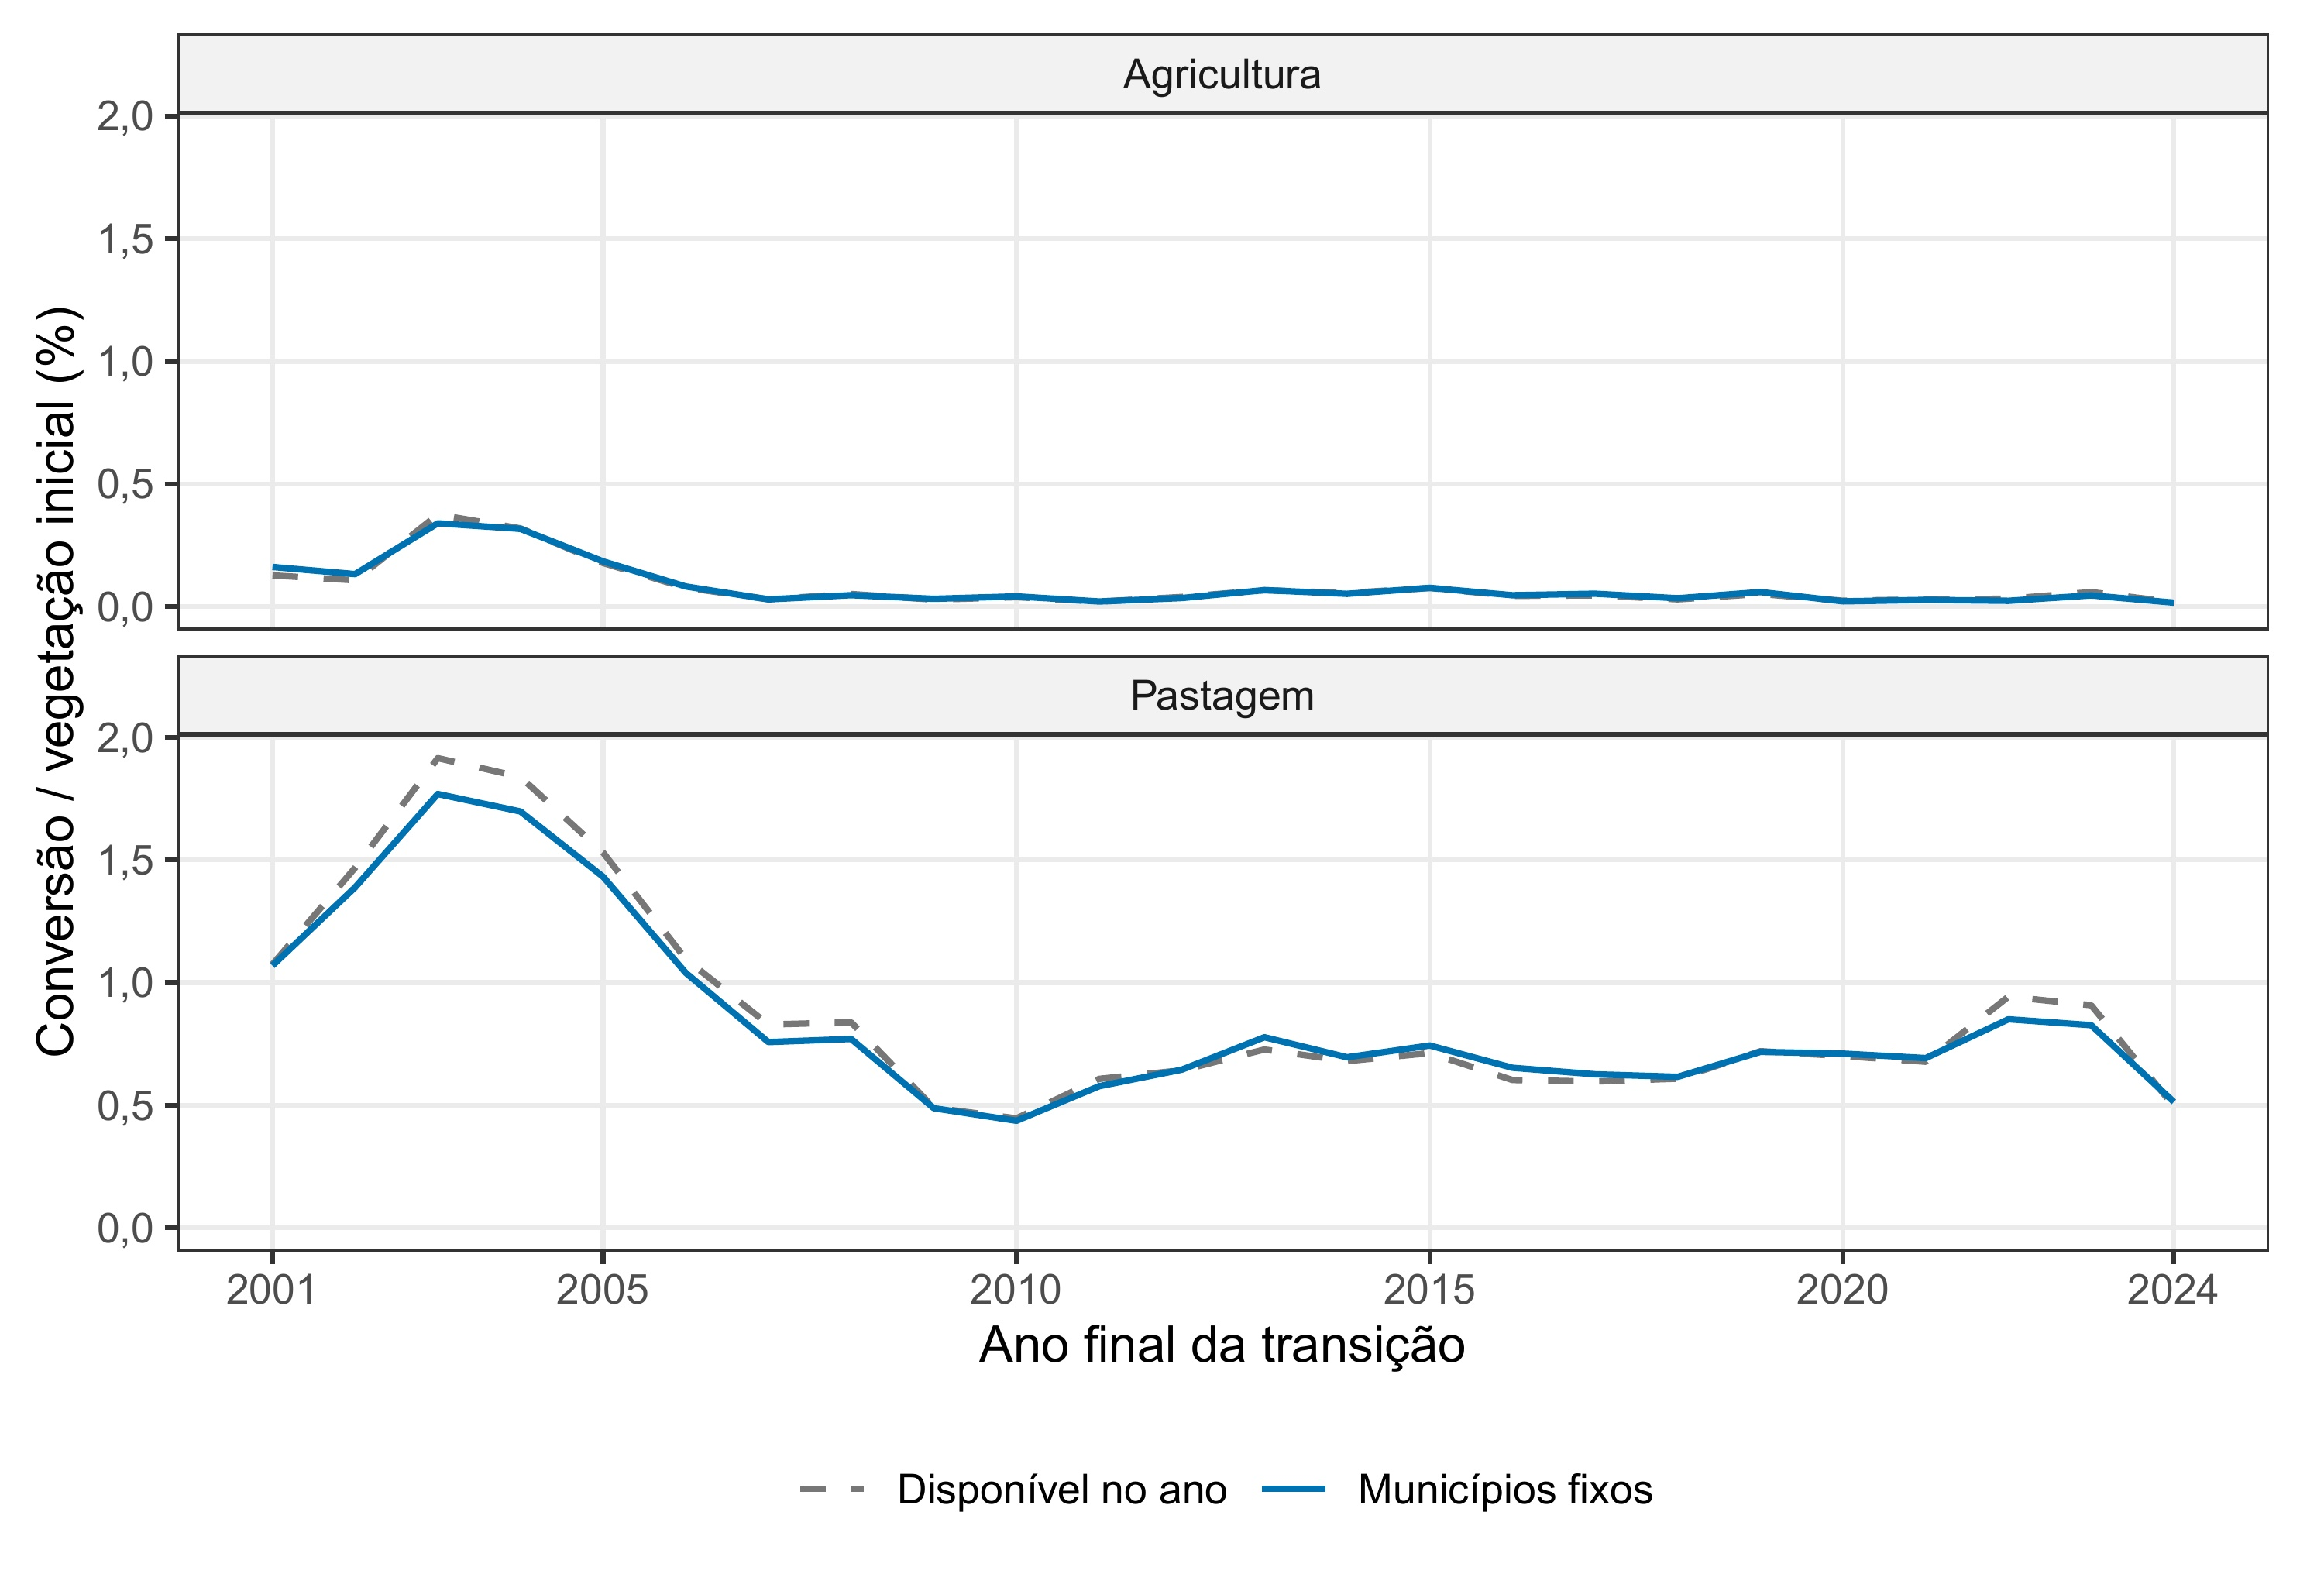
\includegraphics[width=\textwidth]{figuras/figura1.jpg}
\caption{Conversão bruta da vegetação nativa para agricultura e pastagem, 2001--2024}
\label{fig:h1-conversao}
\begin{minipage}{\textwidth}\normalsize\centering
Fonte: elaboração própria com MapBiomas 10.1 e malha IBGE 2023.
\end{minipage}
\end{figure}


Os preços internacionais de soja, milho e carne bovina provêm da \textit{Pink Sheet}. As cotações mensais foram deflacionadas pelo índice de preços ao consumidor urbano dos Estados Unidos (CPI-U) para dólares de poder de compra médio de 2024, exigindo doze meses para cada média anual \cite{WorldBank2026,BLSCPI2026}. A Figura~\ref{fig:h1-precos} apresenta índices com base 100 em 2000, permitindo comparar variações proporcionais entre produtos cotados em unidades diferentes. Os preços de 2000--2023 antecedem as conversões de 2001--2024. Em 2023, as três cotações reais superavam as de 2000, embora as taxas de conversão fossem menores nos extremos correspondentes. Essa comparação descritiva reúne mudanças de contexto e não identifica a resposta condicionada aos preços.

O contraste entre esses extremos não contradiz, por si, a associação mais positiva prevista em H1a: a hipótese compara a resposta entre capacidades locais, mantidas as demais condições, enquanto as séries agregadas reúnem mudanças produtivas, institucionais e de composição. A cotação da carne situa ainda uma alternativa de uso da terra, em diálogo com o problema de preços relativos examinado por \citeonline{Braganca2018}. Sua presença no gráfico contextualiza a comparação, sem transformar as três séries em medidas de rentabilidade ou de retorno recebido pelos produtores mato-grossenses.

\begin{figure}[H]
\centering
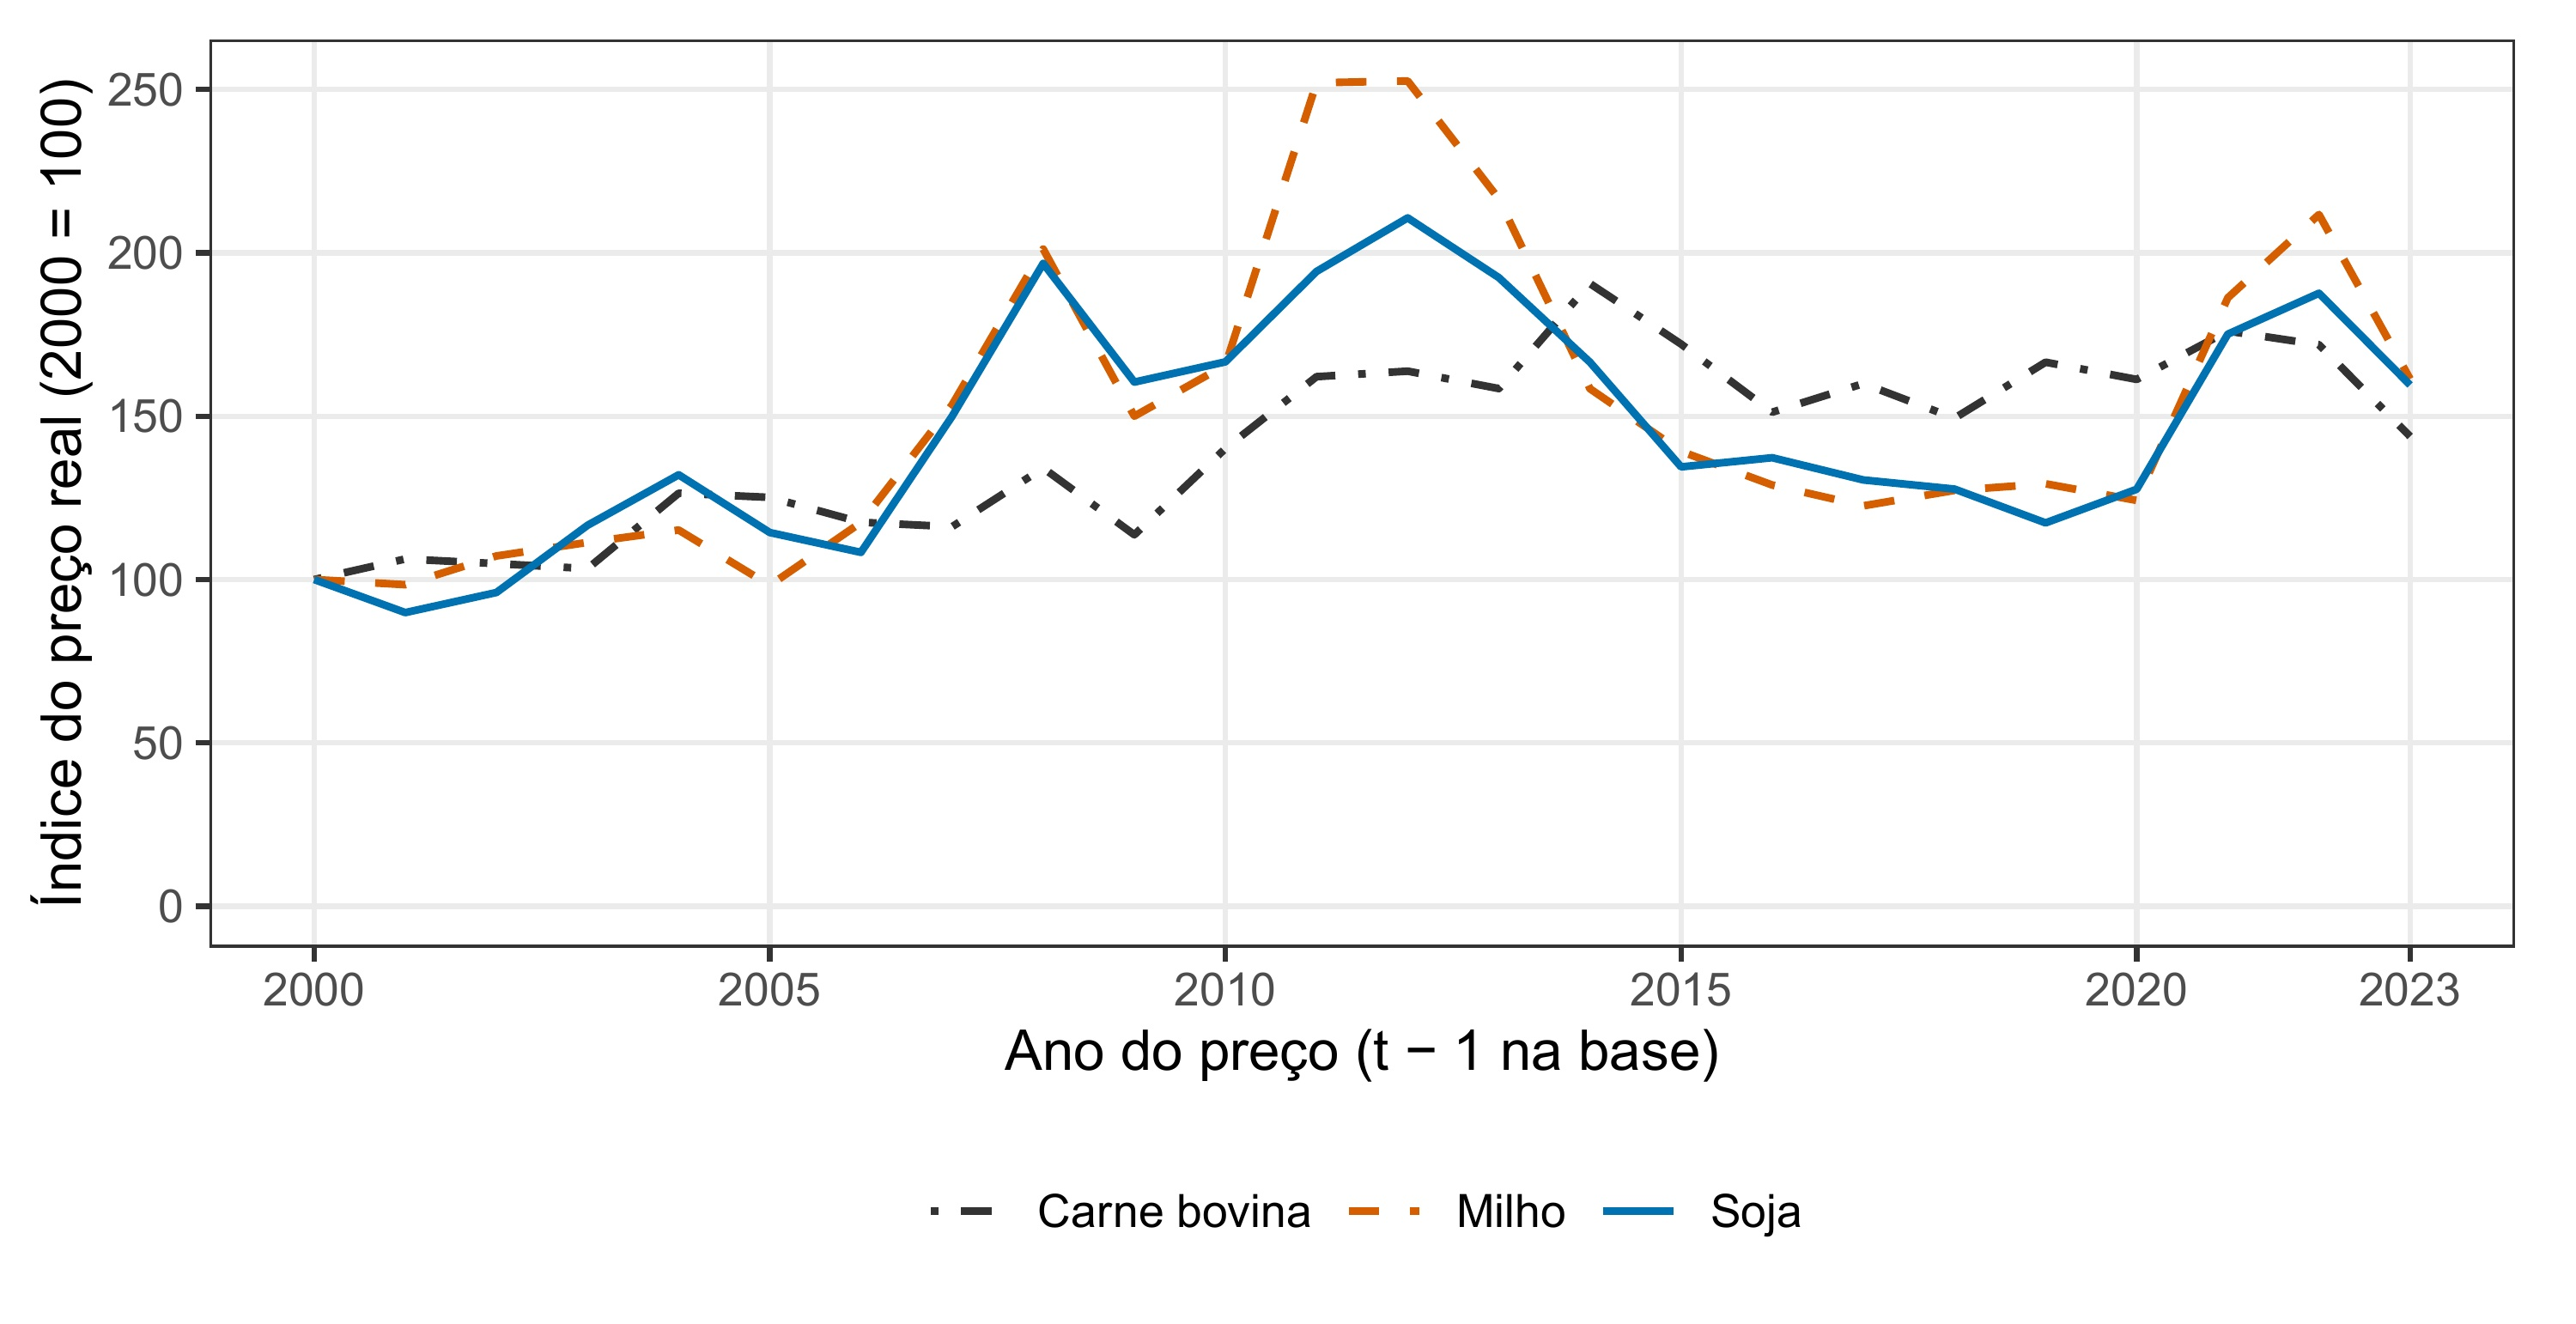
\includegraphics[width=\textwidth]{figuras/figura2.jpg}
\caption{Preços reais internacionais de soja, milho e carne bovina}
\label{fig:h1-precos}
\begin{minipage}{\textwidth}\normalsize\centering
Fonte: elaboração própria com Banco Mundial e CPI-U BLS/FRED.
\end{minipage}
\end{figure}


O potencial agrícola é medido pelo Global Agro-Ecological Zones (GAEZ), versão 4 em sequeiro e alto insumo, em quilogramas de matéria seca por hectare \cite{FAOGAEZ2021}. O indicador da melhor classe de aptidão de cada célula foi agregado por média dos pixels válidos, ponderada pelo cosseno da latitude para aproximar suas áreas. A climatologia é 1961--1990, mas a versão incorpora bases territoriais de 2010. Portanto, o indicador fixo não garante anterioridade de todos os componentes às decisões do painel. Ele descreve possibilidades sob condições padronizadas, sem representar rendimento comercial observado, tecnologia efetivamente empregada ou potencial específico das parcelas nativas disponíveis. O mesmo potencial padronizado é conservado nas diferentes amostras.

Na Tabela~\ref{tab:h1-capacidade}, cada município participa uma única vez. As medianas de potencial para soja e milho são maiores no grupo de predominância Cerrado que no amazônico, mas os intervalos entre os percentis 25 e 75 se sobrepõem. A classificação por bioma, portanto, não substitui a variação produtiva municipal. É essa variação que permite comparar a associação com uma cotação comum entre localidades com possibilidades diferentes, conforme o argumento de H1a. A tabela caracteriza o potencial; não demonstra que os municípios de maior capacidade converteram mais vegetação.

\begin{table}[H]
\centering\normalsize
\setlength{\tabcolsep}{6pt}
\caption{Potencial produtivo municipal por cultura e bioma predominante}
\label{tab:h1-capacidade}
\begin{tabular}{llrrr}
\hline
Cultura & Bioma & Municípios & Mediana & P25--P75 \\
\hline
Soja & Amazônia & 76 & 2.701 & 2.557--2.852 \\
Soja & Cerrado & 61 & 3.261 & 2.817--3.390 \\
Soja & Pantanal & 4 & 3.421 & 3.386--3.457 \\
Milho & Amazônia & 76 & 3.002 & 2.862--3.264 \\
Milho & Cerrado & 61 & 3.320 & 2.797--3.572 \\
Milho & Pantanal & 4 & 6.790 & 6.321--6.933 \\
\hline
\end{tabular}
\par\smallskip\begin{minipage}{\textwidth}\normalsize\centering
Fonte: elaboração própria com FAO/IIASA, GAEZ v4, e IBGE.
\end{minipage}
\end{table}


Os quatro municípios de predominância Pantanal apresentam potencial calculado elevado, especialmente para milho. Esse resultado exige distinguir a média dos pixels válidos no cenário GAEZ da viabilidade do cultivo nas parcelas disponíveis. Como discutido na fundamentação, condições de inundação, usos pecuários e acesso podem limitar a realização do potencial. Tampouco os quatro municípios integram igualmente as amostras de perdas. A diferença entre possibilidade padronizada, cultivo observado e informação suficiente para estimar o modelo impede interpretar a posição desse grupo como recomendação de expansão agrícola no bioma.

O desempenho anterior acrescenta uma dimensão distinta. A produção por hectare plantado reúne o rendimento colhido e a proporção da área plantada que chegou à colheita. Na Figura~\ref{fig:h1b-perdas}, as colunas correspondem a soja e milho, e o eixo horizontal registra a safra anterior. Os painéis superiores dividem a produção total pelas áreas plantada ou colhida dos mesmos municípios elegíveis, enquanto a referência é a média das previsões locais ponderada pela área plantada corrente. Nos painéis intermediários, as perdas médias atribuem igual peso aos municípios, e a frequência divide os casos de déficit de pelo menos 20\% pelo número elegível, mostrado abaixo. A média municipal não é a distância entre as curvas agregadas nem a fração da produção estadual perdida.

\begin{figure}[H]
\centering
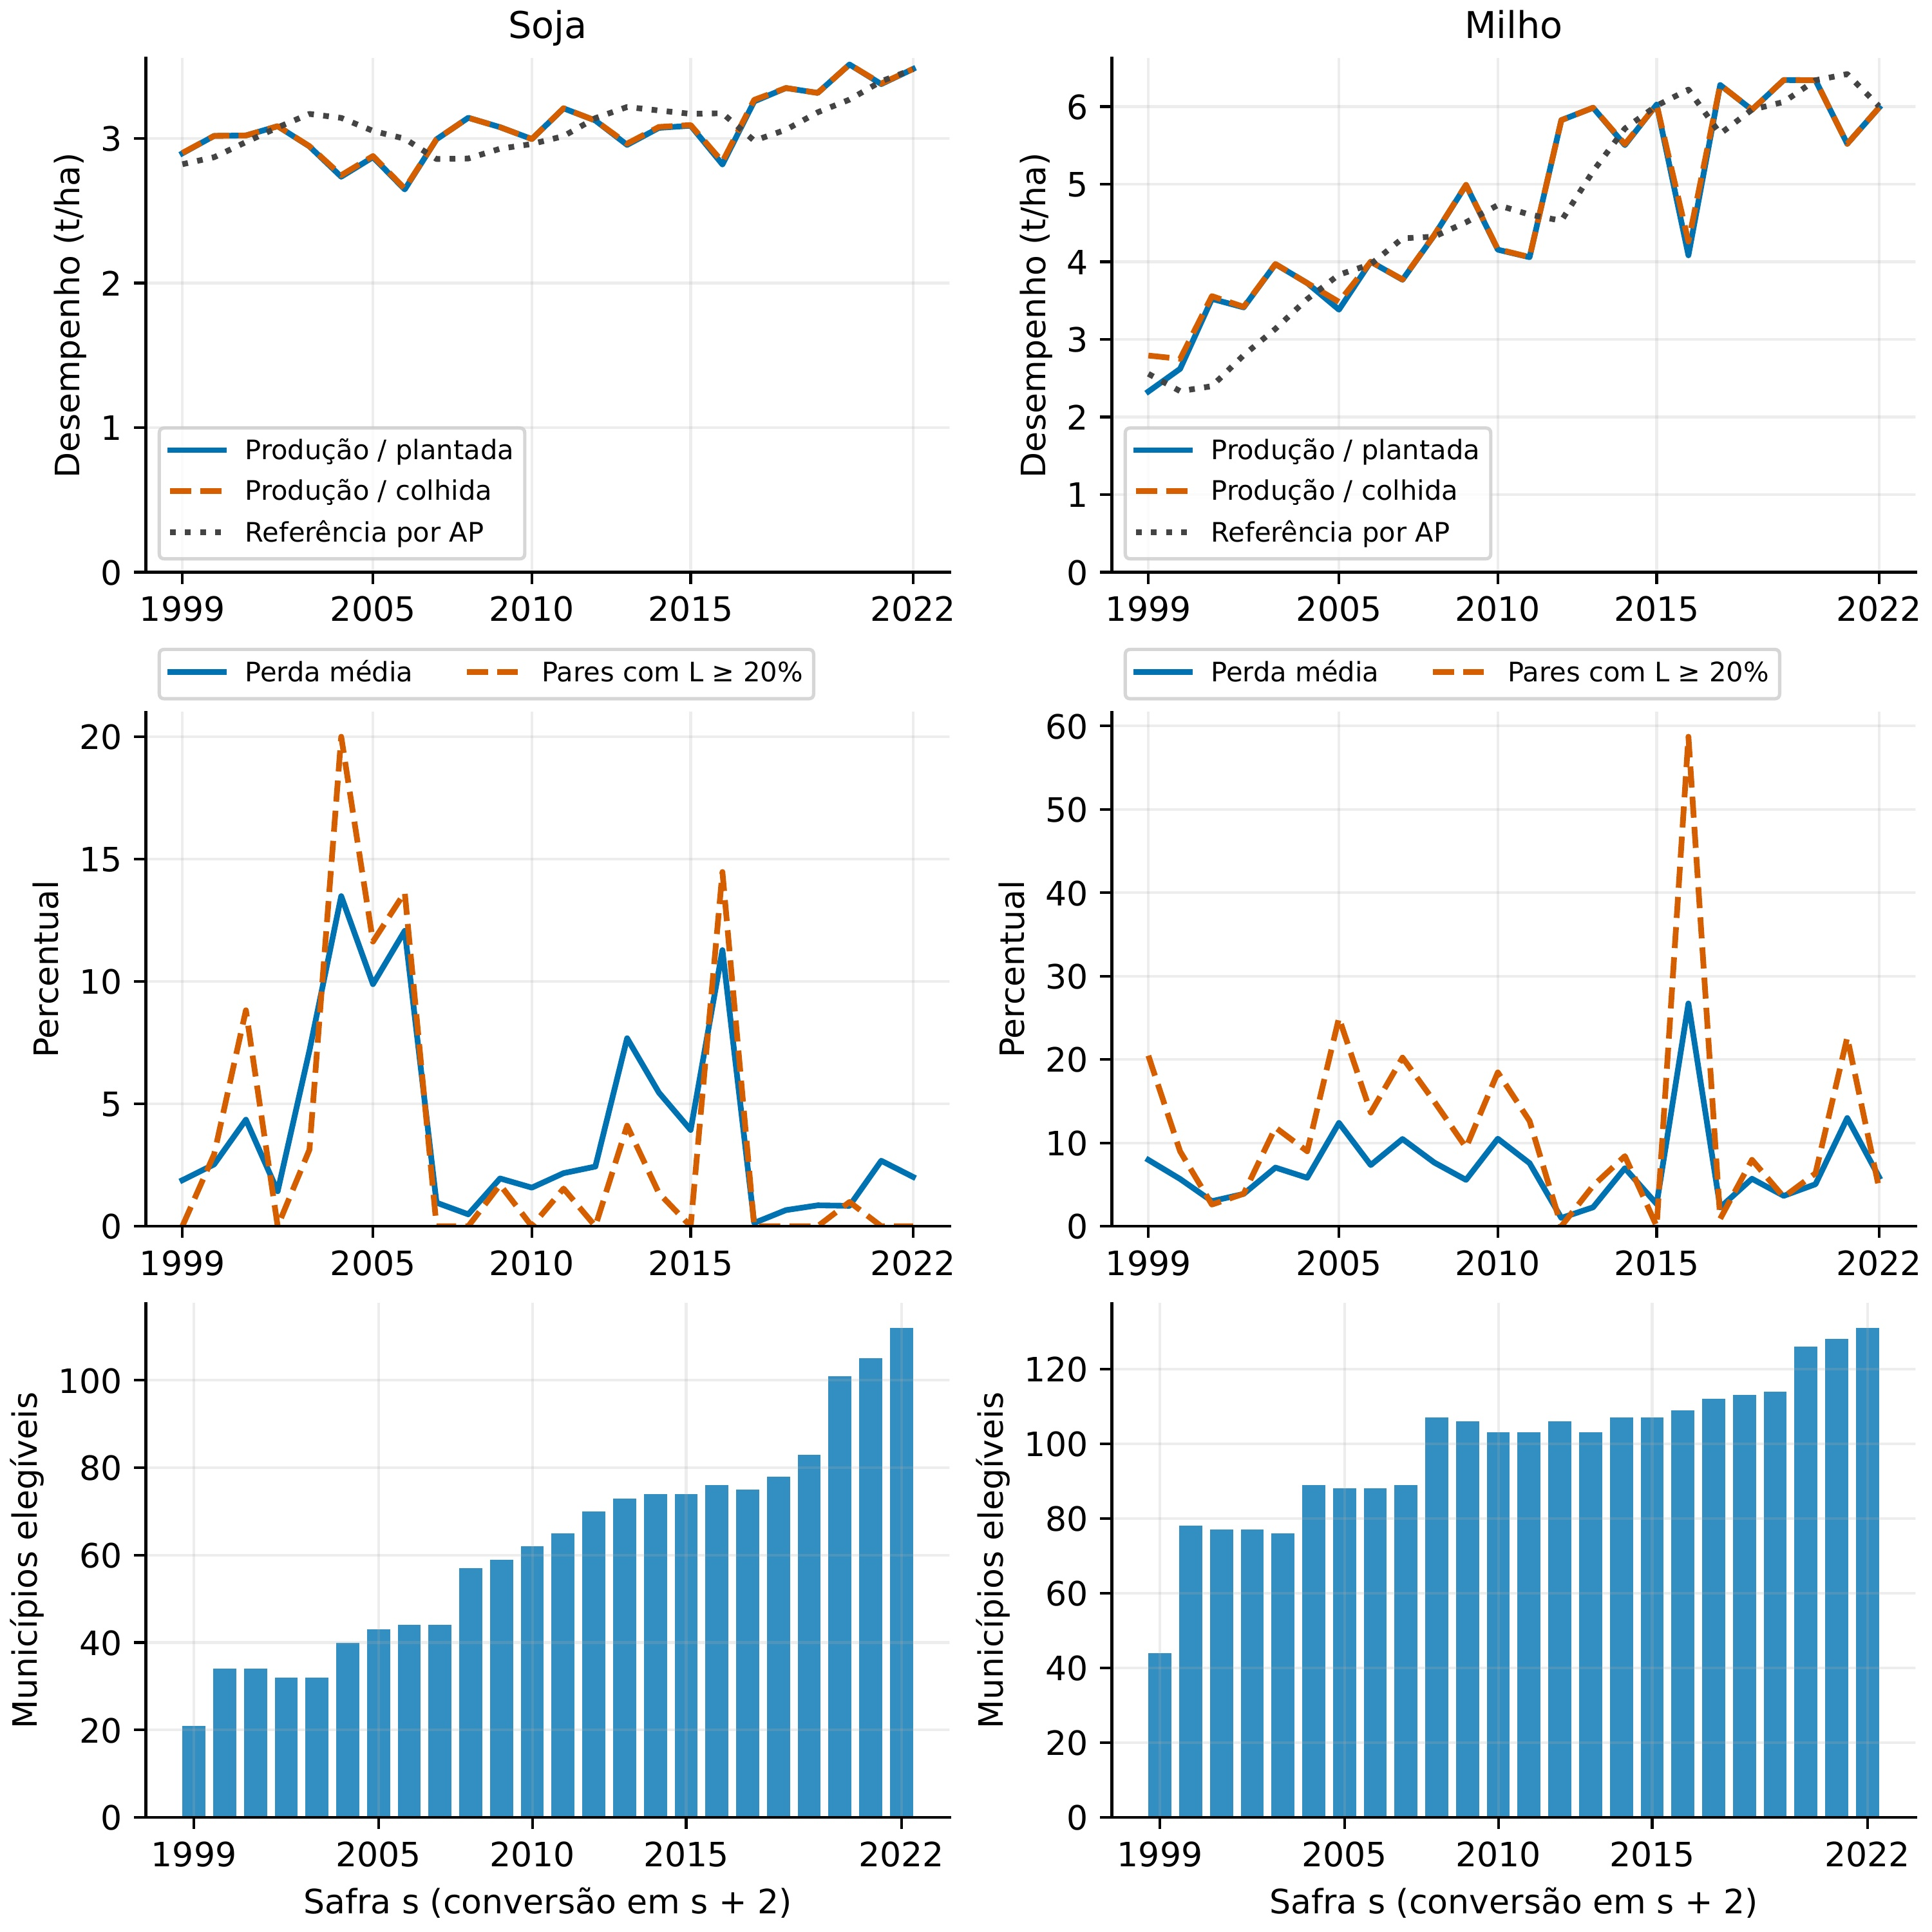
\includegraphics[width=\textwidth]{figuras/figura3.jpg}
\caption{Desempenho agrícola, perdas anteriores e cobertura das amostras ($AP$: área plantada; $L$: intensidade da perda; $s$: safra anual)}
\label{fig:h1b-perdas}
\begin{minipage}{\textwidth}\normalsize\centering
Fonte: elaboração própria com IBGE/PAM e MapBiomas 10.1.
\end{minipage}
\end{figure}


Em 2016, por exemplo, a amostra de milho apresentou 4,08 t/ha plantado e 4,26 t/ha colhido, diante de referência ponderada de 6,22 t/ha. A perda municipal média foi 26,7\%, e 58,7\% dos 109 municípios elegíveis registraram déficit de pelo menos 20\%. A comparação reúne menor desempenho nas áreas colhidas e não colheita de parte da área plantada, sem identificar a causa. No alinhamento principal, essa safra é vinculada ao preço de 2017 e à conversão entre 2017 e 2018. Essa sequência permite perguntar se uma perda anterior acompanha uma associação diferente com o preço subsequente, mas não mede a disponibilidade de recursos nem uma intenção de recuperar a produção por abertura. A cobertura muda entre safras; suas médias não descrevem a evolução do risco em um grupo fixo.

A disponibilidade de histórico também difere entre culturas e territórios. Antes da remoção dos grupos unitários dos efeitos fixos, as perdas válidas da soja cobrem 43,0\% dos pares com conversão observada no grupo amazônico e 63,7\% no Cerrado. No milho, essas proporções são próximas de 86\% nos dois grupos. No Pantanal, há 28 pares elegíveis de soja em dois municípios e 52 de milho em três, número que se reduz na estimação. Em todo o estado, a amostra elegível reúne 42 ocorrências de perda de pelo menos 20\% na soja e 283 no milho. Esses números descrevem o suporte de H1b, não uma comparação de risco entre culturas ou biomas: cultivo, registro e composição diferem, e os pares observados não constituem choques de preço independentes.

Na Tabela~\ref{tab:h1b-composicao}, as médias e medianas atribuem o mesmo peso a cada par município--ano. A coluna observada reúne os 2.772 pares de conversão; soja e milho são subconjuntos sobrepostos com perda anterior válida. As taxas usam o estoque nativo inicial, e os potenciais fixos reaparecem em cada ano observado. A conversão agrícola média é menor nos subconjuntos elegíveis, sobretudo no milho. A tabela antecipa, assim, que incluir perdas modifica também a composição da amostra. A chuva caracteriza outra condição variável no tempo: sua anomalia anual, em milímetros, compara a precipitação com a média municipal de 1981--2000, utilizando a série Climate Hazards Group InfraRed Precipitation with Station data (CHIRPS). Ela não corresponde diretamente ao clima da safra anterior.

\begin{table}[H]
\centering\normalsize\captionstyle{\centering}\normalcaption
\caption{Composição da amostra observada e das amostras com perdas anteriores}\label{tab:h1b-composicao}
\begin{tabular}{p{5.2cm}*{3}{p{3.3cm}}}
\hline
Indicador & Observada & Soja & Milho \\
\hline
Pares município--ano & 2.772 & 1.488 & 2.381 \\
Municípios & 137 & 115 & 137 \\
Conversão agrícola (\%) & 0,112 (0,014) & 0,106 (0,029) & 0,085 (0,013) \\
Conversão para pastagem (\%) & 1,192 (0,799) & 0,943 (0,701) & 1,142 (0,765) \\
Potencial da soja (kg MS/ha) & 2.942 (2.837) & 2.981 (2.950) & 2.965 (2.916) \\
Potencial do milho (kg MS/ha) & 3.245 (3.135) & 3.177 (3.066) & 3.269 (3.144) \\
Anomalia de chuva em t (mm) & -31,4 (-36,4) & -33,3 (-43,7) & -33,3 (-41,2) \\
\hline
\end{tabular}
\par\smallskip\begin{minipage}{\textwidth}\normalsize\centering
Fonte: elaboração própria com MapBiomas, IBGE/PAM, GAEZ v4 e CHIRPS.
\par\medskip
\raggedright Legenda: Médias, com medianas entre parênteses, com igual peso aos pares município--ano. MS: matéria seca. As amostras das culturas se sobrepõem; elegibilidade antecede a remoção de grupos unitários dos efeitos fixos.
\end{minipage}
\end{table}


A seleção pelo histórico conecta a descritiva à interpretação dos resultados. Uma alteração no gradiente preço×capacidade pode decorrer da entrada em uma amostra com menor conversão média, mesmo antes de incluir a perda no modelo. Por isso, a estratégia seguinte compara a especificação sem perdas na amostra original e na amostra comum, para somente então acrescentar os termos de H1b. As diferenças descritivas orientam essa comparação, sem determinar antecipadamente o sinal dos coeficientes.

\label{sec:estrategia}

\subsection{Conversão, perdas e ordenação temporal}

A variável dependente é a taxa anual de conversão bruta da vegetação nativa para agricultura. Para o município $i$ e o ano $t$, divide-se a área dessa transição pelo estoque nativo em $t-1$, multiplicando-se por cem. A unidade é ponto percentual (p.p.) do estoque inicial. A mesma construção define o desfecho complementar de pastagem. Ao observar diretamente as transições, a medida evita que regeneração em outras parcelas compense a abertura do ano, como ocorreria numa diferença líquida entre estoques. O destino registrado é o uso imediatamente posterior à vegetação; a classificação não informa a cultura plantada, a legalidade da abertura ou os agentes que a realizaram.

A quebra é construída separadamente para cada cultura $c$, comparando o desempenho realizado com uma referência histórica municipal. Utiliza-se $r^c_{is}=Q^c_{is}/AP^c_{is}$, em que $Q$ é a produção e $AP$, a área plantada na safra anual $s$. Quando as áreas são positivas, essa razão pode ser escrita como rendimento por hectare colhido multiplicado pela proporção colhida da área plantada. Essa decomposição dá sentido à escolha: um município pode apresentar perda mesmo que o rendimento das parcelas que chegaram à colheita se mantenha. A medida também pode variar com manejo, composição de áreas ou erro de declaração, de modo que seu déficit não equivale automaticamente a dano climático.

A referência $\widehat r^c_{is}$ resulta de uma tendência linear estimada com os dez anos anteriores a $s$, exigindo pelo menos sete observações válidas e previsão positiva. A tendência admite evolução gradual do desempenho, ao passo que a janela móvel limita a influência de um passado produtivo distante. Nenhuma observação futura participa da previsão. Descontinuidades territoriais identificadas reiniciam o histórico, evitando que a mudança da unidade seja interpretada como perda. A intensidade é definida por:
\begin{equation}
L^c_{is}=\max\left\{0,\,1-\frac{r^c_{is}}{\widehat r^c_{is}}\right\}.
\label{eq:perda}
\end{equation}
Assim, $L=0,20$ indica desempenho 20\% abaixo da referência local, e realizações acima dela recebem zero na especificação principal. Ausência de cultivo e informação insuficiente permanecem sem perda calculada. Uma versão binária identifica déficits de pelo menos 20\%; alternativas utilizam tendências de cinco ou quinze anos, com mínimos de quatro ou onze observações, mediana histórica de dez anos com mínimo de sete, área colhida e limiares de 10\% ou 30\%. A referência é uma estimativa, e não uma produtividade que teria sido observada com certeza na ausência de choque.

O alinhamento principal associa a transição dos mapas entre $t-1$ e $t$ à perda da safra $t-2$ e ao preço médio de $t-1$. Para a conversão de 2001, por exemplo, utiliza-se a perda de 1999, cuja referência pode mobilizar 1989--1998, e o preço de 2000. Para 2024, utilizam-se perda de 2022 e preço de 2023. A separação reduz a sobreposição entre o desempenho medido e a abertura que se pretende descrever, mas os dados anuais não permitem ordenar todas as decisões dentro de cada ano. A PAM agrega as safras de milho, e os mapas não datam cada supressão. A alternativa com perda em $t-1$ é, por isso, uma verificação distinta, sujeita a maior sobreposição temporal.

Define-se $p^c_{t-1}$ como o logaritmo do preço real, centrado na média dos 24 valores anuais usados no painel. A capacidade $Z^c_i$ é padronizada pela média e pelo desvio-padrão dos 141 municípios, conservados em todas as amostras. Essa padronização permite comparar coeficientes sem que a unidade de capacidade mude quando municípios são excluídos. Uma variação de 10\% no preço corresponde a $\ln(1,10)$ na escala logarítmica. O modelo em nível do logaritmo relaciona o patamar real do incentivo à conversão; a variação anual e a razão entre preços respondem a perguntas diferentes e entram apenas como alternativas identificadas separadamente.

\subsection{Contrastes de capacidade e perdas}

O núcleo procura distinguir duas formas de heterogeneidade. A primeira compara a associação com preços entre municípios de diferentes capacidades potenciais; a segunda compara essa associação diante de diferentes perdas anteriores. Para cada cultura, estima-se:
\begin{equation}
\begin{split}
y^{ag}_{it}={}&\alpha_i+\lambda_{b(i),t}
 +\beta_c p^c_{t-1}Z^c_i
 +\theta_c L^c_{i,t-2}
 +\delta_c p^c_{t-1}L^c_{i,t-2}\\
 &+\gamma_c Z^c_i\tau_t+\rho_c R_{it}+\varepsilon^c_{it},
\end{split}
\label{eq:nucleo}
\end{equation}
em que $\alpha_i$ são efeitos municipais, $\lambda_{b(i),t}$ são efeitos do bioma predominante por ano, $\tau_t=(t-2001)/10$ e $R_{it}$ é a anomalia anual de precipitação, em centenas de milímetros. Os efeitos municipais absorvem características locais constantes; os de bioma por ano absorvem choques comuns aos municípios de cada grupo no mesmo ano. A tendência diferenciada por capacidade permite que municípios de maior potencial sigam trajetória gradual distinta, além da associação com o preço. A chuva representa uma condição contemporânea que pode afetar diretamente vegetação e conversão, sem ser utilizada como instrumento para a perda.

Os coeficientes $\beta_c$ e $\delta_c$ são comuns aos biomas no núcleo. Os efeitos de bioma por ano condicionam a comparação, mas não correspondem a inclinações próprias para Amazônia, Cerrado e Pantanal. As extensões territoriais descritas adiante examinam outra dimensão, relacionada às frações de exposição e aos marcos institucionais, com os limites de suporte de cada cultura.

Os níveis isolados de preço e capacidade não aparecem porque são absorvidos pelos efeitos fixos. Sua interação continua identificável se houver variação suficiente de capacidade entre municípios e de preços ao longo do tempo, após os demais termos. A perda varia nas duas dimensões e permanece na equação junto com preço×perda. O parâmetro $\theta_c$ descreve sua associação no preço centrado igual a zero; H1b se refere a $\delta_c$, que altera a inclinação em relação ao preço. A presença de uma associação entre perda e conversão, sem essa interação, não seria um teste da sub-hipótese.

Para H1a, o contraste entre municípios separados por um desvio-padrão de capacidade, diante de uma alta de 10\% no preço, é $\beta_c\ln(1,10)$ p.p. A hipótese prevê $\beta_c>0$. Para H1b, a diferença associada a dez pontos percentuais adicionais de perda é $\delta_c\ln(1,10)\times0,10$ p.p.; seu sinal é uma questão empírica. Esses contrastes não recuperam o efeito médio de uma alta de preços em Mato Grosso, absorvido pelos efeitos temporais. Eles descrevem diferenças condicionais de associação, com as demais variáveis da equação mantidas constantes.

A especificação B corresponde à Equação~\ref{eq:nucleo}. A especificação A exclui os dois termos de perda e é estimada tanto na amostra disponível originalmente quanto nas mesmas chaves de B. A comparação entre A original e A comum identifica a alteração associada ao recorte, enquanto A comum e B mostram a alteração decorrente da inclusão dos termos, conservando as observações. A amostra elegível pela perda contém 1.488 pares na soja e 2.381 no milho. A remoção de grupos unitários sem contribuição à estimação com esses efeitos fixos deixa, respectivamente, 1.459 pares em 106 municípios e 2.376 em 134. A original reúne 2.767 pares em 134 municípios. A versão com limiar de 20\% utiliza as mesmas chaves de B.

Essa distinção é relevante para o alcance territorial. No Pantanal, B dispõe de oito pares em dois municípios para soja e cinquenta em três para milho. O painel não fornece base comparável à dos demais biomas para interpretar uma resposta própria dessa região. O histórico também seleciona localidades com cultivo e registro suficientemente contínuos. A análise das perdas diz respeito a esse conjunto, sem representar integralmente municípios de entrada recente na agricultura ou unidades sem informação válida.

\subsection{Inferência e verificações de estabilidade}

A multiplicação dos preços anuais por características municipais amplia a variação das interações, mas não cria novos choques independentes de preço. Apresentam-se três procedimentos de inferência: agrupamento por município, agrupamento simultâneo por município e ano e covariância robusta à heterocedasticidade e à autocorrelação (HAC), com banda dois sobre os escores anuais da regressão completa residualizada. Neste último, a aplicação de Frisch--Waugh--Lovell preserva os coeficientes de B; utilizam-se pesos de Bartlett, sem pré-branqueamento ou ajuste adicional de pequena amostra. Os graus de liberdade são, respectivamente, $G-1$, $\min(G,T)-1$ e $T-1$, em que $G$ é o número de municípios e $T$, o de anos. Com 24 anos, as duas últimas referências utilizam 23 graus de liberdade.

O agrupamento municipal admite dependência serial dentro da unidade; o agrupamento duplo acrescenta dependência entre municípios no mesmo ano. O HAC dos escores anuais examina a persistência temporal da contribuição agregada à estimação. Nenhum procedimento garante acomodar toda forma de dependência espacial e temporal, especialmente com poucos anos e interações concentradas. Por isso, a apresentação conserva a divergência entre as inferências. Intervalos são de 95\%, e ajustes de Holm são aplicados a famílias explicitadas: os dois gradientes H1a de B, separadamente dos dois modificadores H1b. Nas extensões, as famílias acompanham o conjunto de contrastes efetivamente examinado; os intervalos apresentados continuam individuais.

As verificações incluem dezesseis definições por cultura, com variações da referência produtiva, intensidade ou ocorrência da perda, calendário, clima, efeitos temporais, tendência por capacidade, janela e preço. Comparações intermediárias nas mesmas chaves separam, quando necessário, modificação da fórmula de alteração de amostra. Também se examinam exclusões locais e anuais, reamostragem restrita por ano e perturbações da referência histórica. Essas últimas verificam a sensibilidade ao indicador gerado, sem converter sua distribuição em intervalo que incorpore toda a incerteza do desenho.

Como antecedentes de H1a, retomam-se exercícios sem perdas para soja que substituem o potencial de alto insumo pelo rendimento potencial em baixo insumo ou pelo índice de adequação GAEZ em alto insumo. As medidas são padronizadas e interagem com preço e tendência, mantendo conversão agrícola, chuva, efeitos municipais e de bioma por ano, em 2.767 pares. Outro exercício usa a média de 1985--2000 da proporção municipal ocupada por agricultura, calculada com as classes 20, 39, 41 e 62 do MapBiomas, com os mesmos tipos de interação e ajustes. Esses modelos descrevem sensibilidade à medida de exposição, com erros-padrão agrupados por município. Não incorporam a perda nem substituem a comparação de A e B na amostra comum.

Três períodos --- 2001--2005, 2006--2011 e 2012--2024 --- permitem verificar se uma associação agregada esconde trajetórias distintas. Interagem-se os termos de interesse com os períodos, preservando os constitutivos e os ajustes de tendência previstos na especificação. Os testes conjuntos examinam tanto a nulidade dos modificadores quanto sua igualdade entre períodos. São comparações exploratórias: os períodos iniciais contêm poucos preços e poucas perdas intensas, sobretudo na soja. Seu uso não transforma as datas em mudanças exógenas ou em avaliação de políticas.

\subsection{Destinos, incentivos conjuntos e instituições}

A extensão para pastagem conserva fórmula e observações de B. A diferença agricultura menos pastagem é estimada diretamente, de modo que sua variância incorpora a covariância entre os destinos. Outra extensão acrescenta a interação entre capacidade e perda e a interação tripla entre preço, capacidade e perda, permitindo que a modificação de H1b também varie com o potencial. Os dois termos entram juntos para respeitar a hierarquia da interação. Os contrastes condicionais são avaliados na distribuição observada; percentis marginais não asseguram observações em todas as combinações de capacidade e perda.

O preço relativo é $\ln[P^c/(1000P^{carne})]$, com o fator mil compatibilizando cotações por tonelada e por quilograma. Essa medida compara incentivos brutos entre produtos, sem descontar custos. Testa-se a restrição de coeficientes opostos que ela impõe a uma versão com preços separados. Estima-se ainda uma versão conjunta de soja e milho na interseção de 1.450 pares em 105 municípios, mantendo referências individuais nessas mesmas chaves. A correlação de 0,948 entre as séries de preços justifica cautela ao separar sua contribuição, mesmo quando a matriz de interações mantém posto completo.

A exposição territorial à Moratória utiliza a fração municipal no bioma Amazônia interagida com o período desde 2007, com alternativa desde 2006. O pacto foi anunciado em julho de 2006; a alteração do marco de desmatamento para julho de 2008 ocorreu em dezembro de 2014. Nenhuma dessas datas equivale a um início uniforme de cumprimento municipal. A medida representa alcance potencial do compromisso sobre a soja, sem observar fornecedores e transações; para milho, caracteriza heterogeneidade no território alcançado pelo pacto de outra cultura.

Para a reforma do Código Florestal, utiliza-se a fração de formações florestais de 2000 na área municipal total, inclusive municípios com valor zero, combinada ao período desde 2013 e, alternativamente, desde 2012. A medida reúne classes 3 e 6 do MapBiomas e não corresponde a percentual jurídico de Reserva Legal, passivo ou situação cadastral. As extensões institucionais acrescentam, separadamente, as interações de preço e capacidade, ou de preço e perda, com exposição e período posterior, com todos os termos de ordem inferior que não são absorvidos e tendência pela exposição. Sua interpretação depende da variação residual disponível e da possibilidade de outras mudanças acompanharem a exposição e a data.

O desenho permanece associativo. Preços internacionais não medem o retorno líquido recebido localmente; clima, infraestrutura, tecnologia e composição produtiva podem variar junto com as interações. A defasagem da perda ordena medidas, mas não elimina choques persistentes ou decisões anteriores que afetem simultaneamente desempenho e conversão. Controles como crédito, renda e produção posteriores à quebra poderiam representar consequências do próprio evento, alterando o contraste. Fiscalização observada também pode responder à pressão de abertura. Esses limites orientam a escolha do núcleo parcimonioso e a interpretação das extensões, sem supor que acrescentar controles produza automaticamente identificação causal.

\section{Resultados e Discussão}
\label{sec:resultados}
\label{sec:discussao}

\subsection{Composição da amostra e contrastes principais}

A Tabela~\ref{tab:h1-principais} mostra que parte relevante da mudança de H1a antecede a inclusão das perdas. Na soja, o gradiente preço×capacidade passa de 0,08484 em A original a 0,04645 em A comum; no milho, de 0,05188 a 0,03090. Ao acrescentar intensidade e interação, B apresenta valores próximos aos da referência comum. A redução, portanto, não pode ser atribuída integralmente a um ajuste por quebra de safra. Ela acompanha a seleção de municípios e anos com histórico produtivo suficiente, cuja diferença de conversão média já aparecia na análise descritiva.

% Gerado por etapa9/publicar_tabelas.py; fontes e células registradas na auditoria.
\begin{table}[H]
\centering
\normalsize
\setlength{\tabcolsep}{2pt}
\renewcommand{\arraystretch}{1}
\normalcaption\captionstyle{\centering}
\caption{Conversão para agricultura: capacidade e perdas anteriores}
\label{tab:h1-principais}
\begin{tabular}{p{5.2cm}*{3}{p{3.3cm}}}
\hline
Variável & A original & A comum & B: intensidade \\
\hline\multicolumn{4}{l}{\textbf{Soja}} \\
$pZ$ & 0,08484 & 0,04645 & 0,04043 \\
 & (0,03578) & (0,05183) & (0,05307) \\
$L$ & -- & -- & -0,13128 \\
 &  &  & (0,06165) \\
$pL$ & -- & -- & 0,42338 \\
 &  &  & (0,29654) \\
$Z\tau$ & 0,04050 & 0,03728 & 0,03610 \\
 & (0,01444) & (0,02365) & (0,02380) \\
$R$ & -0,01348 & -0,00643 & -0,00650 \\
 & (0,00626) & (0,00437) & (0,00437) \\
Pares município--ano & 2.767 & 1.459 & 1.459 \\
Municípios & 134 & 106 & 106 \\
$R^2$ total & 0,3828 & 0,5109 & 0,5119 \\
$R^2$ \textit{within} & 0,0198 & 0,0159 & 0,0180 \\
\hline\multicolumn{4}{l}{\textbf{Milho}} \\
$pZ$ & 0,05188 & 0,03090 & 0,03218 \\
 & (0,01787) & (0,01823) & (0,01820) \\
$L$ & -- & -- & 0,04491 \\
 &  &  & (0,03955) \\
$pL$ & -- & -- & -0,01315 \\
 &  &  & (0,11571) \\
$Z\tau$ & 0,05382 & 0,05062 & 0,05080 \\
 & (0,01517) & (0,01791) & (0,01781) \\
$R$ & -0,01516 & -0,00322 & -0,00310 \\
 & (0,00671) & (0,00342) & (0,00344) \\
Pares município--ano & 2.767 & 2.376 & 2.376 \\
Municípios & 134 & 134 & 134 \\
$R^2$ total & 0,3807 & 0,4213 & 0,4217 \\
$R^2$ \textit{within} & 0,0165 & 0,0184 & 0,0190 \\
\hline\end{tabular}
\par\smallskip
\begin{minipage}{\textwidth}\normalsize\centering
Fonte: elaboração própria com MapBiomas 10.1, IBGE/PAM, GAEZ v4, Banco Mundial, CPI-U e CHIRPS.
\par\medskip
\raggedright Legenda: $p$: log-preço real centrado; $Z$: capacidade potencial padronizada; $L$: intensidade da perda; $\tau$: tendência em décadas; $R$: anomalia de chuva em centenas de milímetros. Preço em $t-1$ e perda em $t-2$. Erros-padrão municipais entre parênteses. Todas as colunas incluem efeitos municipais e de bioma por ano. A original: amostra disponível; A comum: mesmas chaves de B; B: inclusão de $L$ e $pL$.
\end{minipage}
\end{table}


Os coeficientes estão na escala da equação, e os valores entre parênteses são erros-padrão com agrupamento municipal. Todas as colunas incluem os efeitos municipais e de bioma por ano, a tendência por capacidade e a anomalia de chuva. O $R^2$ total incorpora a contribuição dos efeitos fixos, enquanto o indicador \textit{within} se refere à variação após sua absorção. A comparação desses ajustes entre amostras diferentes não constitui medida de superioridade da explicação econômica. A leitura substantiva se concentra nos contrastes e em sua precisão sob as três inferências.

Em B, os gradientes de H1a continuam positivos nas duas culturas, mas os intervalos de 95\% abrangem zero. O modificador de H1b é positivo na soja e próximo de zero, com sinal negativo, no milho; seus intervalos também abrangem zero nos três procedimentos. A versão binária com limiar de 20\% não produz contraste preciso. A Tabela~\ref{tab:h1-magnitudes} apresenta os intervalos dos contrastes principais. Esses resultados preservam a direção prevista para a capacidade no núcleo, sem confirmar sua positividade de forma geral; para as perdas, não permitem estabelecer uma modificação estável nem concluir que ela inexista.


A associação isolada da perda ajuda a esclarecer a diferença entre nível e interação. Na soja, seu coeficiente é negativo e rejeita zero com agrupamento municipal, mas não com agrupamento duplo ou HAC. Como o preço foi centrado, esse coeficiente se refere à associação da perda no patamar médio do logaritmo do preço. Mesmo que fosse preciso nos três casos, ele não demonstraria restrição financeira nem substituiria o contraste preço×perda. A mudança de precisão reforça a necessidade de distinguir o parâmetro examinado da narrativa que poderia explicá-lo.

% Gerado por etapa9/publicar_tabelas.py; fontes e células registradas na auditoria.
\begin{table}[H]
\centering
\normalsize
\setlength{\tabcolsep}{2pt}
\renewcommand{\arraystretch}{1}
\normalcaption\captionstyle{\centering}
\caption{Contrastes de capacidade e perda para aumento de 10\% no preço (p.p.)}
\label{tab:h1-magnitudes}
\begin{tabular}{p{2.4cm}*{4}{p{3.1cm}}}
\hline
Cultura / hipótese & Estimativa & IC95 mun. & IC95 mun.+ano & IC95 HAC(2) \\
Soja / H1a & 0,00385 & [-0,00618; 0,01388] & [-0,00666; 0,01437] & [-0,00273; 0,01044] \\
Soja / H1b & 0,00404 & [-0,00157; 0,00964] & [-0,00452; 0,01259] & [-0,00517; 0,01324] \\
Milho / H1a & 0,00307 & [-0,00036; 0,00650] & [-0,00139; 0,00752] & [-0,00075; 0,00688] \\
Milho / H1b & -0,00013 & [-0,00231; 0,00206] & [-0,00211; 0,00186] & [-0,00110; 0,00085] \\
\hline\end{tabular}
\par\smallskip
\begin{minipage}{\textwidth}\normalsize\centering
Fonte: elaboração própria com MapBiomas 10.1, IBGE/PAM, GAEZ v4, Banco Mundial, CPI-U e CHIRPS.
\par\medskip
\raggedright Legenda: H1a: um desvio-padrão adicional de capacidade; H1b: dez pontos percentuais adicionais de perda. p.p.: pontos percentuais. IC95: intervalo individual de 95\%. mun.: agrupamento municipal; mun.+ano: agrupamento duplo; HAC(2): covariância robusta à heterocedasticidade e à autocorrelação, banda dois.
\end{minipage}
\end{table}



A Tabela~\ref{tab:h1-magnitudes} traduz os coeficientes para uma alta de 10\% no preço, combinada a um desvio-padrão adicional de capacidade ou a dez pontos percentuais adicionais de perda. Para H1b, os contrastes são 0,00404 p.p. na soja e $-0,00013$ p.p. no milho. Com agrupamento duplo, os intervalos são $[-0,00452;\,0,01259]$ e $[-0,00211;\,0,00186]$ p.p. A unidade refere-se ao estoque nativo inicial, e não à variação percentual da área agrícola. As taxas médias de conversão nas amostras de B são 0,10810 e 0,08506 p.p.; elas contextualizam a escala, mas a divisão de um contraste por essas médias não o transforma em efeito causal proporcional.

A direção positiva dos gradientes de capacidade em B é compatível com a ideia de que uma valorização da cultura aumenta mais a receita potencial por hectare em locais produtivamente favorecidos. A imprecisão, entretanto, impede estabelecer essa relação de forma geral no recorte com histórico. A comparação com \citeonline{BermanEtAl2023} deve considerar que seu desenho, território e suporte de variação diferem dos utilizados aqui. Acrescentar perdas a um painel municipal não constitui, por si só, demonstração de um mecanismo ausente naquele estudo. O avanço específico está na distinção entre capacidade potencial, desempenho anterior e destino da conversão, acompanhada da verificação de quanto o resultado depende da composição e da inferência.

Essa distinção também limita a interpretação tecnológica. O potencial sob alto insumo e sequeiro representa uma possibilidade padronizada; não informa o insumo utilizado nas parcelas convertidas. Nos modelos antecedentes para soja, descritos na metodologia e estimados sem perdas, a associação positiva do cenário de alto insumo não se reproduz sob baixo insumo e se torna negativa com o índice de adequação. A ocupação agrícola anterior apresenta relação distinta do potencial. Esses resultados qualificam a leitura de H1a, em consonância com a heterogeneidade das respostas à intensificação discutida por \citeonline{Spera2017}. Como não incluem o contraste com perdas, permanecem antecedentes de H1a e não evidência de H1b.

\subsection{Estabilidade temporal e informação disponível}

As alternativas não revelam uma definição de perda que sustente H1b uniformemente. Nenhum dos dezesseis modificadores por cultura rejeita zero após o ajuste de Holm, em qualquer das três inferências. Há resultados pontualmente mais precisos: na soja, a janela desde 2006 produz modificador negativo e rejeição bruta no agrupamento duplo e no HAC. Após o ajuste na família, os p-valores passam a 0,5557 e 0,4161. O sinal oposto ao núcleo permanece pertinente, sem orientar a seleção do resultado principal.

A decomposição por períodos explicita essa instabilidade. Na soja, preço×perda é positivo em 2001--2005 e negativo nos dois períodos seguintes; no milho, é negativo no primeiro e pequeno nos demais. Os testes de nulidade conjunta e igualdade dos modificadores rejeitam com HAC após Holm nas duas culturas, sem uniformidade entre os procedimentos. Para H1a, o gradiente da soja em 2012--2024 é negativo, com intervalo de agrupamento duplo inteiramente abaixo de zero. Esse resultado contraria a direção da sub-hipótese naquele recorte e deve acompanhar a interpretação dos sinais positivos do núcleo. Nesse período, o coeficiente é $-0,04995$, com intervalo de $[-0,08465;\,-0,01524]$.

A informação desses contrastes está distribuída de forma desigual. Os períodos iniciais contêm cinco e seis preços anuais, e a soja reúne apenas cinco ocorrências de perda de pelo menos 20\% no primeiro. Na inferência HAC, mudar a banda entre zero e quatro mantém as rejeições brutas dos testes da soja; no milho, elas dependem da banda. Em B, Jangada em 2013, associada à safra de 2011, concentra 29,85\% da soma de quadrados residualizada de preço×perda da soja. Excluir esse par eleva o modificador, ainda impreciso; retirar 2003 muda seu sinal. A influência é documentada sem eliminar observações para obter uma direção desejada.

As verificações adicionais mantêm a incerteza. A reamostragem restrita por ano, com 999 replicações, produz p-valores de 0,603 e 0,877 para os modificadores de soja e milho. Nas 499 perturbações da referência histórica por cultura, os quantis de 2,5\% e 97,5\% também atravessam zero. São sensibilidades condicionais à construção do indicador, não intervalos que resolvem toda a incerteza. Na alternativa que substitui o preço defasado pelo futuro, o gradiente preço×capacidade do milho é positivo nas três inferências. Esse comportamento, limitado ao período com preço futuro disponível, recomenda cautela diante de tendências persistentes; não demonstra antecipação ou expectativa dos produtores.

A formulação sem sinal prévio de H1b encontra respaldo na diversidade de respostas possíveis, e não na equivalência de todas as explicações. Uma quebra pode reduzir recursos próprios, alterar acesso ao crédito e adiar investimento; também pode ser seguida de expansão se houver condições para financiar a atividade ou reorganizar a produção. O painel não observa essas decisões nem identifica qual restrição foi determinante. Por isso, o sinal positivo da interação na soja não prova recuperação de renda por abertura, assim como o sinal negativo em recortes posteriores não demonstra falta de liquidez. Essas interpretações permanecem hipóteses sobre processos que poderiam produzir as associações.

Essa leitura também delimita a comparação com \citeonline{OrdonezEtAl2025} e \citeonline{HsiaoEtAl2026}. Seus resultados de expansão após choques adversos não implicam que a interação entre uma cotação internacional e uma perda anterior deva ser positiva em Mato Grosso. De modo semelhante, as associações entre lucros setoriais e perda florestal encontradas por \citeonline{RichardsArima2026} não são diretamente comparáveis ao modificador de uma perda física municipal. O indicador deste artigo não observa o saldo financeiro da safra. A contribuição do contraste é mostrar o alcance e a precisão dessa relação específica, preservando como questões abertas a transmissão aos recursos e a escolha entre alternativas de uso da terra.

Para integrar risco agrícola e conservação, uma extensão futura precisaria observar a transmissão entre perda, recursos e decisões sobre a terra. Dados de seguro, crédito contratado, custos e receitas poderiam distinguir exposição produtiva de capacidade financeira, desde que sua posição temporal fosse explícita. Incluir renda ou crédito realizados depois da perda como controles pode retirar justamente parte do caminho que se deseja estudar. O desenho atual fornece critérios para organizar essa investigação, sem apresentar como efeito de política uma associação que ainda depende de choques omitidos e seleção de amostra.

\subsection{Destinos e extensões do contraste}

A Tabela~\ref{tab:h1-destinos-robustez} compara agricultura e pastagem nas mesmas observações de cada cultura. Os gradientes preço×capacidade são maiores para pastagem. A diferença entre destinos é imprecisa na soja e rejeita zero nos p-valores brutos das três inferências no milho. Neste último caso, +10\% no preço e um desvio-padrão adicional de capacidade correspondem a uma diferença de $-0,04315$ p.p. entre os gradientes de agricultura e pastagem. Na família de quatro contrastes, contudo, o p-valor ajustado permanece abaixo de 5\% apenas com agrupamento municipal. As diferenças de preço×perda são imprecisas mesmo antes do ajuste.

% Gerado por etapa9/publicar_tabelas.py; fontes e células registradas na auditoria.
\begin{table}[H]
\centering
\normalsize
\setlength{\tabcolsep}{2pt}
\renewcommand{\arraystretch}{1}
\normalcaption\captionstyle{\centering}
\caption{Gradientes por destino da conversão e diferença entre destinos}
\label{tab:h1-destinos-robustez}
\begin{tabular}{p{3.4cm}p{2.0cm}p{3.9cm}p{2.0cm}p{3.9cm}}
\hline
Destino & $\beta$ & IC95 de $\beta$ & $\delta$ & IC95 de $\delta$ \\
\hline\multicolumn{5}{l}{\textbf{Soja}} \\
Agricultura & 0,04043 & [-0,0699; 0,1508] & 0,42338 & [-0,4743; 1,3211] \\
Pastagem & 0,21472 & [-0,0065; 0,4360] & 0,28650 & [-3,2205; 3,7935] \\
Agricultura--pastagem & -0,17429 & [-0,4297; 0,0811] & 0,13688 & [-4,0375; 4,3112] \\
\hline\multicolumn{5}{l}{\textbf{Milho}} \\
Agricultura & 0,03218 & [-0,0145; 0,0789] & -0,01315 & [-0,2218; 0,1955] \\
Pastagem & 0,48490 & [0,0647; 0,9051] & -1,18909 & [-3,6083; 1,2302] \\
Agricultura--pastagem & -0,45272 & [-0,8824; -0,0231] & 1,17594 & [-1,2361; 3,5879] \\
\hline\end{tabular}
\par\smallskip
\begin{minipage}{\textwidth}\normalsize\centering
Fonte: elaboração própria com MapBiomas 10.1, IBGE/PAM, GAEZ v4, Banco Mundial, CPI-U e CHIRPS.
\par\medskip
\raggedright Legenda: $\beta$: coeficiente de preço×capacidade; $\delta$: coeficiente de preço×perda. IC95: intervalo individual de 95\%, com agrupamento municipal e anual. Mesmas chaves de B por cultura. A diferença entre destinos é estimada diretamente, incorporando sua covariância.
\end{minipage}
\end{table}



Os intervalos dessa tabela utilizam agrupamento por município e ano. O potencial permanece o da cultura, inclusive na equação de pastagem. A comparação permite reconhecer que os dois destinos apresentam associações diferentes em algumas especificações, sem converter capacidade agrícola em capacidade pecuária. Também não acompanha o deslocamento de atividades entre parcelas ou municípios.

A interação tripla com capacidade não torna H1b mais conclusiva. Seus coeficientes são positivos na soja e negativos no milho, mas nenhum dos seis testes da família rejeita após Holm nas três inferências. Os contrastes condicionais nos percentis de capacidade têm intervalos de agrupamento duplo que abrangem zero. Os intervalos dos gradientes com preço relativo à carne também abrangem zero. As restrições de coeficientes opostos não são rejeitadas, o que não estabelece equivalência entre medidas. Na amostra compartilhada pelas culturas, a inclusão conjunta não produz rejeição dos testes conjuntos de H1a ou H1b.

A comparação entre destinos ajuda a compreender por que produção e conversão não caminham necessariamente juntas. A substituição de pastagens por lavouras pode ampliar a produção sem abertura imediata de vegetação, enquanto novas pastagens podem surgir em outras áreas. \citeonline{MacedoEtAl2012} documentaram a importância de terras previamente abertas para a expansão da soja na porção florestal de Mato Grosso; \citeonline{Braganca2018} mostrou que preços relativos podem se associar a reorganização de usos sob condições particulares. O maior gradiente da pastagem em parte das estimativas é compatível com a relevância de examinar esses destinos em conjunto, mas não identifica a sequência de realocação descrita por tais mecanismos. As interdependências discutidas por \citeonline{SimoesEtAl2020} e \citeonline{JungEtAl2022} exigem informações que ultrapassam o destino municipal imediato.

\subsection{Heterogeneidade em torno dos marcos institucionais}

Nas datas principais, nenhum dos oito contrastes institucionais rejeita após Holm com agrupamento municipal ou duplo. No HAC, a interação de preço, perda, fração amazônica e período desde 2007 para o milho é negativa e mantém rejeição ajustada, assim como a alternativa desde 2006. Para +10\% no preço, +0,10 na perda e +0,10 na fração amazônica, o primeiro contraste equivale a $-0,00891$ p.p. na diferença pós--pré. A rejeição restrita ao HAC é apresentada como parte da evidência, sem ser tomada como concordância entre procedimentos. Para a data principal, os p-valores ajustados são 1,00000, 0,14054 e 0,00212, respectivamente, com agrupamento municipal, agrupamento duplo e HAC.

A variação que sustenta esse contraste está concentrada. Depois dos demais termos, permanece apenas 0,453\% da soma de quadrados da interação do milho após os efeitos fixos; um município concentra 19,0\% da variação parcial, e 2005, 41,9\%. As dezesseis matrizes institucionais de agrupamento duplo e a do modelo conjunto exigiram correção de autovalores negativos. O procedimento conserva os coeficientes e viabiliza os intervalos, mas não amplia a informação disponível. Na comparação pela cobertura florestal inicial em torno de 2012, o contraste H1a da soja é negativo, com rejeições brutas que não persistem após Holm.

A divergência inferencial no contraste do milho ilustra esse problema. A rejeição ajustada no HAC deve constar da interpretação, mas diz respeito à associação de perdas e preços num território potencialmente alcançado pelo pacto da soja. Não constitui efeito direto da Moratória sobre a comercialização de milho. A concentração da variação residual e a necessidade de corrigir matrizes de covariância reforçam o cuidado com sua precisão. Da mesma forma, o contraste pela floresta inicial não informa o custo de adequação ao Código em cada imóvel. Seria inadequado utilizar essas estimativas para concluir que uma das políticas conteve ou ampliou a resposta às quebras.

Essa delimitação não contradiz a evidência de conservação identificada por outros desenhos. \citeonline{HeilmayrEtAl2020} avaliaram a Moratória em áreas aptas à soja, e \citeonline{HardingEtAl2021} investigaram o condicionamento da resposta aos preços sob instrumentos de conservação. A comparação exige reconhecer diferenças no tratamento, na unidade de exposição e no contrafactual. Um efeito médio de redução da abertura pode coexistir com mudanças na sensibilidade aos incentivos; o presente artigo não dispõe da identificação necessária para separar essas duas relações como efeitos causais das políticas. Sua contribuição institucional é explicitar o alcance das medidas territoriais e o suporte empírico das interações.

\subsection{Implicações para a gestão ambiental}

Para a gestão ambiental, a implicação é acompanhar o caminho da expansão, além do volume produzido. O crescimento da safra pode resultar de rendimento, frequência de cultivo, substituição de uso ou incorporação de novas áreas; cada margem envolve pressões distintas. Uma leitura apoiada apenas em produção ou área agrícola líquida pode reunir processos opostos. Os dados de transição bruta oferecem uma medida mais próxima da abertura observada, mas ainda precisam ser relacionados às parcelas, à sequência de usos e às regras aplicáveis para sustentar decisões operacionais. O artigo não estima um limiar de preço para acionar fiscalização nem classifica municípios por risco previsto.

A utilidade gerencial dos resultados está, portanto, na organização de dimensões que precisam ser observadas conjuntamente. Preços situam os incentivos; capacidade e desempenho descrevem possibilidades e experiências locais; transições brutas mostram o destino imediato da abertura; informações por imóvel e cadeia permitiriam relacioná-los às obrigações e aos compromissos comerciais. A integração dessas dimensões pode orientar o desenho de monitoramento e a formulação de perguntas verificáveis. As estimativas apresentadas não estabelecem a eficácia de uma combinação específica de crédito, seguro e fiscalização, nem sustentam recomendações uniformes para os três biomas.

Por fim, a comparabilidade deve acompanhar qualquer uso territorial da evidência. O Pantanal possui suporte muito reduzido no núcleo, enquanto os municípios de cultivo recente podem ser excluídos pela falta de histórico. A alteração da amostra ao longo dos anos exige separar mudança econômica de mudança na informação disponível. Para além de Mato Grosso, essa é uma contribuição metodológica pertinente a regiões em que expansão agrícola, risco produtivo e conservação coexistem: reconhecer quem e quais decisões entram no contraste antes de transferir seu resultado para uma política. A validade dessa transferência depende das instituições, das alternativas de uso e da qualidade das observações em cada contexto.

\section{Conclusões}
\label{sec:conclusao}

O artigo examinou a associação dos preços reais de soja e milho com a conversão bruta da vegetação nativa para agricultura em Mato Grosso, considerando a capacidade produtiva potencial, as perdas anteriores e condicionantes territoriais. A distinção entre produzir mais e abrir novas áreas orientou tanto a descrição quanto a comparação com pastagens. O painel combinou informações de transição, produção, potencial agronômico, preços e clima, preservando a diferença entre capacidade, desempenho realizado e resultado econômico.

A exigência de histórico para construir perdas alterou a composição da amostra e reduziu os gradientes preço×capacidade antes da inclusão dos termos de H1b. No núcleo, os sinais de H1a permaneceram positivos, mas imprecisos; os modificadores associados às perdas também apresentaram intervalos que abrangem zero nas três inferências. Esses resultados não confirmam as sub-hipóteses de forma geral nem demonstram ausência das associações propostas. As comparações por período, destino e exposição acrescentaram heterogeneidade, inclusive resultado contrário à direção de H1a, cuja interpretação depende do suporte e do tratamento da dependência.

As perdas físicas não identificam, isoladamente, restrições financeiras ou intenção de compensar receita por expansão. Da mesma forma, frações territoriais e datas institucionais não medem cumprimento nem permitem atribuir os contrastes ao Código Florestal ou à Moratória. A conexão entre ambiente, condições locais e sequência temporal permanece pertinente, com o alcance empírico delimitado pelas variáveis observadas. Uma defasagem organiza a comparação, sem demonstrar planejamento intertemporal.

Para a gestão ambiental, o estudo reforça a necessidade de acompanhar destinos da abertura, condições produtivas e cobertura da informação de forma articulada. O crescimento da produção não basta para inferir pressão de conversão, e uma associação municipal não define a resposta de cada produtor. Avançar na ligação entre risco agrícola e conservação requer observar a transmissão das perdas aos recursos e às decisões sobre a terra, além das obrigações e dos compromissos por imóvel ou cadeia. Essas informações permitiriam avaliar instrumentos específicos, preservando as diferenças entre os biomas e as alternativas efetivamente acessíveis aos produtores.

\bibliographystyle{abntex2-alf}
\bibliography{citation-options,library}
\end{document}
